\documentclass[ijoc,sglanonrev]{informs4}

\usepackage{url}
\usepackage{graphicx}
\usepackage[T1]{fontenc}
\usepackage[algo2e,linesnumbered,ruled]{algorithm2e} 
\usepackage{appendix}
\usepackage{tabularx}       % automatic column width
\usepackage{mathtools}  
\usepackage{amsfonts}       % mathbb
\usepackage{xfrac}          % slanted fractions
\usepackage{bm}             % bold greeks 
\usepackage [autostyle, english = american]{csquotes} % left and right opening quotes with "
\usepackage{wrapfig}        % text flows around image
\usepackage{array}          % Needed for custom column types
\usepackage{xcolor}
\colorlet{added}{blue!80!black} 
\usepackage{setspace}       % for controlled interline
% \usepackage{lineno}
\usepackage{enumitem}
%\usepackage{caption}
%\usepackage[labelfont=sf]{subcaption}
%\captionsetup{subrefformat=parens,font=footnotesize}
%\subcaptionsetup[figure]{textfont=sf,position=bottom}
\usepackage{eqndefns-left} % For checking the display equation width and equation environment definitions %
%\RequirePackage{tgtermes}
%\RequirePackage{newtxtext}
%\RequirePackage{newtxmath}
%\RequirePackage{endnotes}
%\usepackage{subfig}         % two aligned subfigures


%\OneAndAHalfSpacedXI
\OneAndAHalfSpacedXII % Current default line spacing
%%\DoubleSpacedXI
%%\DoubleSpacedXII

% Optional LaTeX Packages
%\usepackage{algorithm}
%\usepackage{algpseudocode}
%\usepackage{tikz}
% Private macros here (check that there is no clash with the style)

% Natbib setup for author-number style
\usepackage{natbib}
 \bibpunct[, ]{(}{)}{,}{a}{}{,}%
 \def\bibfont{\small}%
 \def\bibsep{\smallskipamount}%
 \def\bibhang{24pt}%
 \def\newblock{\ }%
 \def\BIBand{and}%

%% Setup of the equation numbering system. Outcomment only one.
%% Preferred default is the first option.
\EquationsNumberedThrough    % Default: (1), (2), ...
%\EquationsNumberedBySection % (1.1), (1.2), ...

%% Setup of theorem styles. Outcomment only one.
%% Preferred default is the first option.
\TheoremsNumberedThrough     % Preferred (Theorem 1, Lemma 1, Theorem 2)
%\TheoremsNumberedByChapter  % (Theorem 1.1, Lema 1.1, Theorem 1.2)
\ECRepeatTheorems  %  

% For new submissions, leave this number blank.
% For revisions, input the manuscript number assigned by the on-line
% system along with a suffix ".Rx" where x is the revision number.
\MANUSCRIPTNO{IJOC-0001-2024.00}
% Redefine X column in tabularx to center the content
\newcolumntype{C}{>{\centering\arraybackslash}X}

%% the following for reducing space around figures
\setlength{\intextsep}{4pt}
\setlength{\textfloatsep}{4pt}
\setlength{\textfloatsep}{4.0pt plus 2.0pt minus 2.0pt}
%\captionsetup{belowskip=0pt}
\setlist[itemize]{noitemsep,nolistsep}

\MakeOuterQuote{"}
\def\UrlFont{\rmfamily}

%%%%%%%%%%%%%%%%
\begin{document}
%%%%%%%%%%%%%%%%

% Outcomment only when entries are known. Otherwise leave as is and
%   default values will be used.
%\setcounter{page}{1}
%\VOLUME{00}%
%\NO{0}%
%\MONTH{Xxxxx}% (month or a similar seasonal id)
%\YEAR{0000}% e.g., 2005
%\FIRSTPAGE{000}%
%\LASTPAGE{000}%
%\SHORTYEAR{00}% shortened year (two-digit)
%\ISSUE{0000} %
%\LONGFIRSTPAGE{0001} %
%\DOI{10.1287/xxxx.0000.0000}%

% Author's names for the running heads
\RUNAUTHOR{Fenga and Maniezzo}

% Enter the (shortened) title:
\RUNTITLE{Bootstrap Enhanced Scenario Optimization}

% Enter the full title:
\TITLE{Bootstrap Enhanced Scenario Optimization, a Case Study in Two-Echelon Logistics for Large-Scale Retail}

\ARTICLEAUTHORS{%
\AUTHOR{Livio Fenga}
\AFF{Center for Simulation, Analytics and Modelling, University of Exeter Business School, \EMAIL{l.fenga@exeter.ac.uk}}

\AUTHOR{Vittorio Maniezzo}
\AFF{Department of Computer Science, University of Bologna, \EMAIL{vittorio.maniezzo@unibo.it}}
} 

\ABSTRACT{%
%(1) Research Questions and Challenges;
We present a data-driven approach to scenario generation based on empirical distributions derived from univariate data series forecasts. The method is demonstrated using a real-world case study of supply chain optimization at the tactical level, focusing on the final stage of two-echelon logistics support for a large retail chain. The problem is modeled as a single-stage stochastic problem and framed as a prescriptive analytics case.
%(2) Methodology and Results;
Our approach uses Maximum Entropy Bootstrap (MEB) with bagging for univariate time series forecasting to predict demand scenarios that incorporate the inherent uncertainties of short, non-stationary time series data. These scenarios are then integrated into a deterministic equivalent model to optimize inventory allocation across distribution centers. The result is accountable and optimized prescriptions for inventory quantification and warehouse floor sizing.
%(3) Importance and Implications.
Our findings, which are also validated against an extended benchmark set of artificial instances, demonstrate the significant value of integrating MEB-enhanced forecasting with scenario-based optimization. They also provide the basis for a forecast-and-optimize framework, called Bootstrap Enhanced Scenario Optimization (BESO), whose generality extends beyond the specific use case.
}%

%\FUNDING{This research was supported by [grant number, funding agency].}
%Supplemental Material:
%Data Ethics & Reproducibility Note:

\KEYWORDS{Stochastic programming, forecasting, Two-echelon logistics, Maximum Entropy Bootstrap, Short time series, Combinatorial optimization} 
%\HISTORY{Received: Month DD, YYYY; Accepted: Month DD, YYYY; Published Online: Month DD, YYYY}

\maketitle
%%%%%%%%%%%%%%%%%%%%%%%%%%%%%%%%%%%%%%%%%%%%%%%%%%%%%%%%%%%%%%%%%%%%%%

% Text of your paper here


\section{Introduction} \label{Sec:intro}

Decision-making under uncertainty is a pervasive challenge in operations research, particularly in complex systems such as logistics networks. Scenario-based optimization has long been used to address this challenge by capturing the variability of future events through a finite set of possible outcomes. However, the reliability of such methods depends heavily on how accurately these scenarios represent the underlying stochastic processes. In this paper, we propose a novel method — Bootstrap Enhanced Scenario Optimization (BESO) — that integrates bootstrap-based forecasting with scenario-based linear optimization to improve the robustness and realism of stochastic modeling. A new data-driven method for empirically estimating the distribution of stochastic variables and embedding it in scenario generation for robust and stochastic optimization may offer significant advantages over standard distribution-aware approaches. Traditional methods often rely on strong assumptions about the underlying probability distribution — typically normality or other parametric forms — which may not accurately reflect the true behavior of real-world uncertainties. In contrast, data-driven techniques directly leverage historical or observed data to construct empirical distributions, capturing nuances such as asymmetry, multimodality, or heavy tails that standard models might miss. This increased fidelity can lead to more realistic and effective scenario generation, improving both the robustness and relevance of the resulting optimization solutions. Furthermore, by adapting to the structure present in the data, data-driven approaches are naturally more flexible and can better accommodate nonstationarities or structural changes in the stochastic environment.

The BESO framework leverages bootstrapped time series to generate diverse and data-driven future scenarios, which are then embedded within constrained stochastic optimization problem, in which a stochastic objective function is optimized, possibly subject to robust, worst-case constraints. Unlike traditional stochastic programming methods that may rely on assumptions of distributional form or limited scenario diversity, BESO incorporates the empirical structure and seasonality of historical data to generate richer and more representative scenario sets.

To demonstrate the practical value and performance of BESO, we apply the method to a real-world two-echelon logistics network problem. In this setting, uncertain outbound freight demands must be managed across multiple depots and customer zones. By using BESO to define demand scenarios and solve for optimal routing and allocation decisions, we show how the method improves both solution robustness and operational efficiency compared to conventional techniques.

The remainder of the paper is structured as follows: Section \ref{Sec:literature} reviews related work in scenario optimization and bootstrap forecasting. Section \ref{Sec:forecasting} presents the BESO methodology in detail. Section \ref{Sec:testcase} describes the case study and implementation. Section \ref{Sec:results} discusses the results, and Section \ref{Sec:conclusions} concludes with key insights and future research directions.

% This paper describes an application of prescriptive analytics in the optimization of a 2-echelon logistics network, with a strong emphasis on the predictive component. The primary objective is to develop and validate a {\it prescriptive analytics framework} of general validity, which is applied here to improve effectiveness in inventory management, customer allocation and demand forecasting within a 2-echelon system. 

% The paper reports on a case study that requires integrated forecasting and optimization for inventory location and retailer allocation in a two-echelon system managed by an LSRT group. The case involves different distribution centers (DCs) and several retailers, each of which maintains its own inventory. DCs act as buffer points between manufacturers/suppliers and lower-tier retailers, and have bulk storage capacity that must be sufficient to hold enough stock to meet demand forecasts. 

% DC dimensioning constituted the primary research objective. This objective is predicated upon the prior determination of necessary inventory levels, calculated by assessing the expected retailers demand and requisite goods availability during a period of the year when criticality is likely to occur. A model was developed to optimize the distribution of goods, which subsequently provides the necessary data to compute DC capacity. The core problem to solve is therefore to determine the total amount of goods to be managed by each DC, which will be split and forwarded to each allocated retailer. Allocations are determined on the basis of advance demand information, which is derived from forecasts based on time series data relating to requests issued by retailers. 

% The test case deals with one of the subproblems that arise when optimizing a 2-echelon logistics chain. In fact, three subproblems are typically identified, namely {\it Facility Location Problem} (FLP) \citep{DH04}, which asks to determine where to locate hubs or distribution centers and which is mainly relevant at the strategic level, Allocation Problem (AP) \citep{KSI13}, which asks to determine which center will service each client, and which is mainly relevant at the tactical level, and Vehicle Routing Problem (VRP) \citep{TV14}, which is about how to define the service routes once the customers of each center have been identified, which is mainly relevant at the operational level. 

% A preliminary work using the same data as this test case was presented in \citep{MZ23}, but with a completely different processing that did not consider bootstrapping and its stochastic/robust optimization integration. In this paper, we therefore propose a completely different and novel approach that greatly expands the significance of the test case. The results obtained on an extended benchmark set are also completely new.

% The proposed forecasting module, contrary to the previous work, is now based on a bootstrap scheme suitable for dependent data (see, e.g., \citep{kreiss2011bootstrap}), a well-known but often neglected methodology that exhibits interesting properties from a managerial perspective and whose comparative effectiveness is also empirically demonstrated by the results we report. Our methodology uses univariate time series forecasting with Maximum Entropy Bootstrap (MEB) and bagging to predict demand, effectively addressing challenges posed by short, non-stationary time series data.

% Univariate time series forecasting focuses on predicting future values of a single variable, which is crucial for industries relying on accurate demand predictions. The MEB method generates resampled datasets that capture the probabilistic structure of the original time series, maintaining its inherent uncertainties, particularly when data is limited.

% Bagging, or bootstrap aggregating, enhances predictive performance by training multiple models on bootstrapped samples and aggregating their predictions, helping to reduce overfitting. This approach also effectively handles the non-stationarity of time series data, allowing us to adapt to changing patterns and produce more reliable demand forecasts.

% Furthermore, a methodological innovation supported by the use of bootstrap forecasting is the possibility to seamlessly combine it with a deterministic equivalent approach for a subsequent linked stochastic optimization problem, giving rise to a forecast-and-optimize framework called Bootstrap Enhanced Scenario Optimization (BESO) whose validity extends beyond the specific case study presented.

% The core problem at the heart of the optimization module is a split assignment problem \citep{B81}, which has been extensively studied in the context of survivable network design, much less so in a logistics context. In this study, we present a computational analysis of the fitness landscape as it applies to logistics, yielding results for dimensions larger than those reported in any other application area.

% The rest of this paper is organized as follows: Section \ref{Sec:literature} reviews the relevant literature on 2-echelon logistics and predictive analytics, with special emphasis on the forecasting component, Section \ref{Sec:testcase} introduces the specific test case presented in this work. The analytical framework we propose is innovative with respect to both the forecasting module, described in section \ref{Sec:forecasting}, and the optimization module, described in section \ref{Sec:optimization}. Section \ref{Sec:results} discusses the results of applying this framework to the case study and to an extended benchmark set of instances to validate the generality of the approach, while section \ref{Sec:conclusions} offers conclusions and suggestions for future research.



\section{Literture review} \label{Sec:literature}

The paper intersects different research threads, both in terms of the theoretical contribution and the application use case.

\subsection{Scenario-Based Robust Optimization}

Stochastic programming has long served as a fundamental framework for modeling decision-making under uncertainty. The early foundations of stochastic programming primarily considered expected-value models and recourse formulations \cite{B55,D55}. In contrast, robust optimization \cite{BN98,BS04} proposes to reformulate the model to a deterministic optimization problem where constraints consider a worst-case outcome. As research matured, hybrid models emerged paying attention to the interplay between constraint satisfaction and objective optimization, with major applications in fields such as energy systems, finance, supply chain management, and transportation planning.

A primary branch is Chance-Constrained Programming (CCP, also Chance-Constrained Optimization) \cite{CC59,P95} where uncertain constraints must be satisfied with at least a prescribed probability level, i.e., they must be satisfied for a high percentage of possible uncertain outcomes, rather than absolutely all of them. The survey in \cite{KJ22} provides an overview of CCP, considering also cases with limited distributional information and discussing reformulations based on sampling and distributional robustness.

On the contrary, hard-constrained stochastic programming \cite{BL11,SDR09} refers to models in which certain constraints must be satisfied in all cases, regardless of the realization of uncertain parameters. These constraints can for example represent physical, safety, or regulatory requirements. The nomenclature tends to be less normative in these cases, but usually when there is some tolerance on constraint violation the name becomes Robust chance-constrained optimization \cite{RM22} and distributionally robust chance constraints when the distribution itself is uncertain \cite{DY10,RM22}. The name distributionally robust optimization (DRO) is also used when looking for the solution most resilient against the worst case probability distribution for the uncertain parameters \cite{DY10}. DRO has been proposed and applied in various logistics and supply chain contexts \cite{WC20,JWCZ22}.

A primary approach to stochastic programming is Scenario-Based optimization. This approach addresses uncertainty by discretizing the continuous probability distribution of uncertain parameters into a finite set of specific {\it scenarios}, each with an associated probability. The optimization problem is then formulated to find decisions that perform well across this set of scenarios.

The Sample Average Approximation (SAA) method is a pivotal technique that addresses this \cite{SH98}. SAA approximates the true underlying distribution with an empirical distribution derived from a sample of independent and identically distributed realizations, i.e., scenarios. By replacing the expectation with a sample mean, the original stochastic problem can be transformed into a deterministic equivalent problem that can then be solved using standard techniques.

The optimization framework of interest for this paper, where we seek to minimize expected costs while ensuring that constraints are satisfied across all generated scenarios, belongs to the category of scenario-based robust optimization. This area is of significant scientific interest. Recent contributions include \cite{CSX20}, a paper introducing the Robust Stochastic Optimization Made Easy (RSOME) framework. This integrates scenario-tree-based stochastic linear optimization with distributionally robust optimization, and is available as a GitHub package \cite{CX23}. \cite{LCKZ23} addresses the stochastic inventory routing problem by integrating scenario-based methods with distributionally robust optimization. It focuses on handling uncertainties in demand by considering various scenarios and ensuring robust solutions that perform well across these scenarios, and \cite{WAJ23} proposes a scenario-based robust optimization approach that combines elements of stochastic programming and robust optimization. This approach emphasizes constructing probabilistic scenarios and protecting against adversarial perturbations within discrete uncertainty sets.

\subsection{Forecast and optimize}

There is a growing body of literature that combines time series forecasting with scenario-based optimization, where typically time series generates forecast paths that become scenario sets.
This integration goes by different names, including predict-then-optimize, stochastic programming with forecast scenarios, Forecast-informed optimization or Scenario-based stochastic optimization.

The typical workflow of these contributions goes through a forecasting phase, using time series models such as SARIMA, GARCH, LSTM, Prophet, XGBoost, etc. to generate point forecasts and/or predictive distributions, followed by a scenario generation phase that simulate or sample possible future paths based on forecasted distributions and finally embed the scenarios into a stochastic program (single or multi-stage) \cite{R18,FTW18,BK19} and more recently into adaptive robust optimization solutions \cite{BB23}.

It is worth noting that the sequential paradigm, where forecasting models first estimate future parameters and the resulting  predictions are then used in optimization models, has been recently questioned. This approach may lead to suboptimal decisions when prediction errors significantly affect the optimization outcomes.
Recent research propose framework, where forecasting models are trained not solely to minimize predictive error but also to improve downstream decision quality \cite{DAK17,WDT19}. Here, the optimization objectives are embedded into the training loss of forecasting models, optimizing decisions directly with respect to the performance in the target optimization problem.

% Robust Stochastic Approximation Approach to Stochastic Programming
% Authors: B. Verweij, S. Ahmed, A.J. Kleywegt, G. Nemhauser, A. Shapiro
% Publication: SIAM Journal on Optimization
% Citation: Verweij, B., Ahmed, S., Kleywegt, A.J., Nemhauser, G., Shapiro, A. (2003). The sample average approximation method applied to stochastic routing problems: A computational study. Comput. Optim. Appl., 24, 289–333.
% Link: SIAM Journal on Optimization 1
% Optimal Robust Optimization Approximation for Chance Constrained Optimization Problem
% Authors: Li, G., Floudas, C.A.
% Publication: ScienceDirect
% Citation: Li, G., Floudas, C.A. (2014). A posteriori probability bounds on constraint violation/satisfaction for robust optimization. Computers and Chemical Engineering.
% Link: ScienceDirect 2
% Optimal and Robust Methods for Stochastic Optimization
% Authors: B. T. Polyak
% Publication: ResearchGate
% Citation: Polyak, B. T. (1997). Optimal and robust methods for stochastic optimization.
% Link: ResearchGate 3
% Stochastic Programming and Robust Optimization
% Authors: Golub, B., Holmer, M., McKendall, R., Pohlman, L., Zenios, S.A.
% Publication: SpringerLink
% Citation: Golub, B., Holmer, M., McKendall, R., Pohlman, L., Zenios, S.A. (1995). Stochastic programming models for money management. European Journal of Operational Research, 85, 282–296.
% Link: SpringerLink 4
% Robust Optimization Approximation for Joint Chance Constrained Optimization Problem
% Authors: Luedtke, J.R., Ahmed, S., Nemhauser, G.L.
% Publication: Journal of Global Optimization
% Citation: Luedtke, J.R., Ahmed, S., Nemhauser, G.L. (2010). An integer programming approach for linear programs with probabilistic constraints. Math. Program., 122(2), 247–272.
% Link: Journal of Global Optimization 5

\subsection{Data-Driven Empirical Distribution Estimation}

Data-driven approaches to estimating the distribution of stochastic variables have gained increasing attention as alternatives to classical parametric modeling, particularly in settings where assumptions of stationarity or known distributional forms are invalid. Unlike traditional techniques that rely on a priori specification of distribution families (e.g., Gaussian or Poisson), data-driven methods infer distributional characteristics directly from historical or observed data, making them especially suited for real-world applications with complex, noisy, or limited information.

Among the most prominent techniques are resampling-based methods such as the Bootstrap \cite{b1}, which generates empirical distributions by repeatedly sampling from the data with replacement. The Maximum Entropy Bootstrap \cite{Vinod2006} extends this idea by producing replicates that preserve dependence structures in time series data, making it particularly valuable for short or non-stationary sequences.

Recent work has explored the integration of these empirical distribution estimates into stochastic and robust optimization pipelines. Notable contributions include nonparametric scenario generation \cite{BM11}, distributionally robust optimization using empirical Wasserstein distances \cite{EK17}, and hybrid models that combine forecasting and optimization in a unified framework \cite{BK19}. 


\subsection{2-echelon logistics networks}

Multi-echelon inventory management is a supply chain control strategy that coordinates inventory across multiple levels, called "echelons," of the chain \citep{Clark60}. Each echelon — typically identified as suppliers, manufacturers, distribution centers, and retailers — may hold inventory. The objective is to optimize inventory across all levels of the supply chain rather than addressing each level in isolation. The literature on this strategy has expanded significantly, covering various aspects such as inventory control policies, replenishment strategies, and inventory risk management, among others. The implementation of effective forecasting and optimization processes represents a fundamental element of a well-defined and effective management policy. 

Forecasting, particularly demand forecasting, has garnered considerable attention in this field \citep{Shenstone01}. Different forecasting paradigms have been proposed \citep{Syntetos05,Keneley02,Ma15}, demonstrating that accurate demand forecasts can be achieved by analyzing historical data and that it is possible to integrate these insights into management models. 

% For example, \citep{A01} provides insights into how predictive analytics and collaborative forecasting can improve the performance of multi-echelon supply chains by anticipating demand and aligning inventory levels across different echelons, while \citep{VAD12} discusses the application of predictive analytics for inventory management in multi-echelon logistics systems, focusing on SKU classification and demand forecasting to optimize inventory levels across different echelons. Other examples can be found in \citep{R97,P16,BS17}. Predictive analytics intersects with big data and Industry 4.0, enabling logistics companies to anticipate trends, manage risk, and make informed decisions. \citep{WGNP16,HR17}. 

The extant literature comprehensively examines diverse facets of multi-echelon inventory management, encompassing inventory control policies, replenishment strategies, and risk mitigation frameworks. Nevertheless, precise demand forecasting, especially within the context of dynamic retail environments characterized by fluctuating trends and seasonal variations, remains a significant obstacle. Multi-echelon demand forecasting commonly employs time series analysis, incorporating a variety of models.  However, the efficacy of these methods frequently hinges on assumptions of stationarity and specific distributional characteristics, which are often violated in empirical data. 
Moreover, the accuracy of demand forecasts demonstrably influences the efficacy of subsequent optimization procedures, thereby highlighting the critical need for robust forecasting methodologies. 

Bootstrap methods can enhance the performance of various machine learning models, including Multilayer Perceptrons (MLP) and Long Short-Term Memory (LSTM) networks. While these methods generally do not require strong distributional assumptions, they can benefit from the application of bootstrap techniques, as these can improve model robustness and mitigate overfitting, addressing concerns that are especially prevalent in scenarios with limited data availability. Studies demonstrate that integrating bootstrap methods with MLP and LSTM significantly improves predictive accuracy \citep{efron1994introduction,hastie2009elements,cho2014learning}. 

% Turning to optimization of two-echelon logistics systems, we see again that a large number of mathematical models have been proposed \citep{Gumus10,Dai17,TGM23}. The primary concern revolves around demand, which is often assumed to be stochastic or specified as stationary. The goal of the optimization process is typically to develop a mathematical model that quantifies the total system cost, possibly enabling the determination of the optimal lot size to be ordered and the reorder point at each level of the supply chain

A  model proposed in \citep{Axsater00} deals with a two-level inventory system that integrates a central warehouse with a number of different retailers, whose  demand was generated by a compound Poisson demand, analogously \citep{Andersson00} studied a two-level inventory system model with a central warehouse and multiple non-identical retailers.
A multistage supply chain model based on Autoregressive Integrated Moving Average (ARIMA) time-series models has been presented in \citep{gilbert2005arima}. It establishes that the orders and inventories at each stage are also ARIMA processes, given an ARIMA model of consumer demand and associated lead times.
Recent developments introduce heuristic approaches for cost optimization, with seasonal or cyclical demands  \citep{Sakulsom19}, or multi-objective optimization and vehicle synchronization \citep{ANHC21}.

Effective multi-echelon inventory management is widely recognized for minimizing the average total cost of inventory by promoting coordination and cooperation among supply chain members. 
%A decentralized inventory policy can indeed lead to excess inventory without enhancing customer service levels \citep{Gumus10}. 
In terms of allocating stores to distribution centers (DCs), each time a DC makes an allocation decision, it can seek advance demand information to reduce uncertainty and associated costs. This approach allows the DC to update its market forecast and anticipate the structural attributes of the model, ultimately providing valuable management insights \citep{P16}.
The majority of cases documented in the literature regarding the implementation of such multi-echelon inventory policies are based on examples of instances with generic demand, generated according to a variety of distributions \citep{Escorcia20,EG81}. The following sections present a real-world use case in which all instance elements are derived from actual records.

% The increasing complexity of large-scale retail trade (LSRT) supply chains has led to an increase in the need for efficient logistics, and this is particularly true in the area of multi-echelon distribution systems. A 2-echelon logistics network, characterized by two levels of supply chain entities, plays a critical role in ensuring the timely and cost-effective delivery of goods. It is a complex system involving interdependent factors such as inventory management, transportation costs, demand variability, and service level requirements. Optimizing these networks is critical for companies seeking to minimize costs while maintaining high service levels, and the study of multi-echelon supply chains with periodic review ordering policies has long prompted specific lines of research \citep{A01,Clark60}. 

% In recent years, {\it predictive analytics} \cite{S10,Si13} and {\it prescriptive analytics} \cite{BK19,PH15} have emerged as powerful tools for improving decision making in various domains, including logistics \citep{DJS18}. By leveraging historical data and forecasting modules, possibly including machine learning and statistical models, prescriptive analytics enables organizations to anticipate trends, identify potential risks, and support informed decisions \citep{HR17,KS17}. It is therefore one of the primary tools to be considered for optimizing the supply chain. 
Specifically, in the context of 2-echelon logistics optimization, prescriptive grounded in predictive analytics is known to provide benefits by refining demand forecasting, inventory allocation, transportation planning, and related decisions \citep{VAD12,KK10,A01}.

Despite the acknowledged benefits, the application of prescriptive analytics in 2-echelon logistics systems is still an area of research and presents several challenges, including how to deal with uncertainties in demand and supply, how to properly model historical series, and how to efficiently formalize the related management decision processes to be supported. 

% Flores et al. (2014), "A Scenario-based Stochastic Model for Supply Chain Planning under Demand Uncertainty"
% Mula et al. (2006), "Mathematical programming models for supply chain production and transport planning"

%%%%%%%%%%%%%%%%%%%%%%%%%%%%%%%%%%%%%%%%%%%%%%%%%%%%%%%%%%%%%%%%%%%%%%%%%%%%%%%%%%%%%%%%
\section{The 2-echelon test case} \label{Sec:testcase}

Our proposed test case comes from an LSRT company that manages multiple retail stores in a large city in northern Italy. Among these, 52 stores provided aggregate sales time series data spanning at least 45 months prior to the forecast period, which is set at a three-month horizon, as detailed in the following. Each store maintains a small inventory, replenished by deliveries from one of four different distribution centers (DCs) in the area. The products are categorized into three lines: fresh, dry, and household. In this context, the focus has been exclusively on the logistics of dry goods, including product categories ranging from personal care items to basic electronics, from household goods to holiday decorations. For this product line, DCs are required to maintain an aggregate inventory sufficient to cover a demand for a period of two weeks.
The supply chain consists of a large distribution center (DC) in the northern suburbs, a smaller DC in the south, and two small satellite facilities closer to the city center. While the satellites have limited storage capacity, they offer lower-cost and more timely service to the majority of the city's stores. Figure \ref{fig:locations}:a shows the (anonymized) geolocation of the DCs and stores and \ref{fig:locations}:b the GIS model of the locations (see also \citep{MZ23}), where the DCs are the orange triangles and the stores are the azure blobs whose size is proportional to the corresponding request.

\begin{figure}[ht]
\centering
\begin{minipage}{0.48\textwidth}
    \centering
    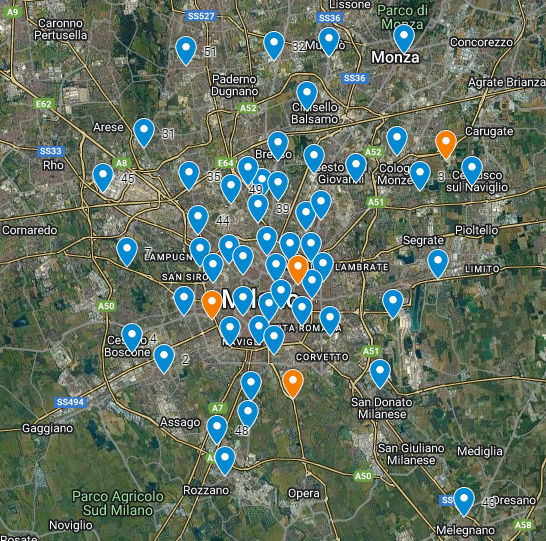
\includegraphics[width=\linewidth]{gmap.png}
    \vspace{0.5em}
    \textit{(a) gmap view}
\end{minipage}
\hfill
\begin{minipage}{0.48\textwidth}
    \centering
    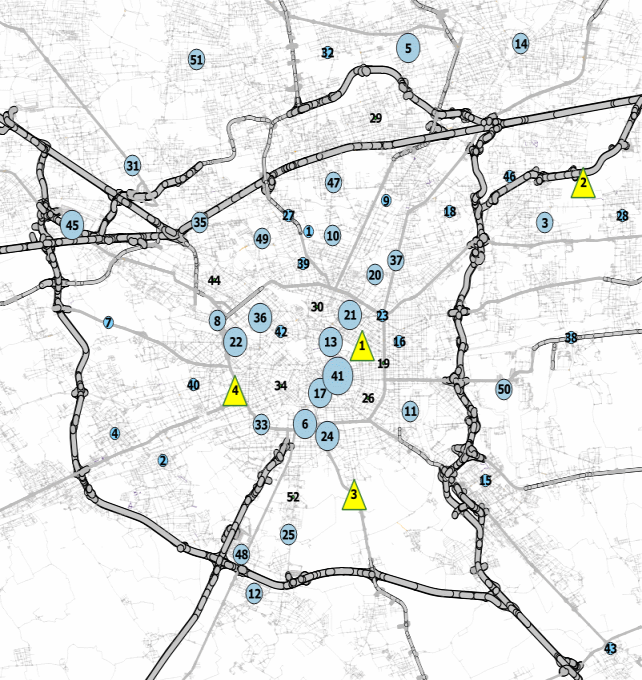
\includegraphics[width=\linewidth]{qgis.png}
    \vspace{0.5em}
    \textit{(b) GIS view}
\end{minipage}
\caption{Stores and distribution centers locations.}
\label{fig:locations}
\end{figure}

Each store must be allocated to a distribution center (DC), ensuring that the total requests made to a DC do not exceed its storage capacity. Both capacities and requests are quantified in terms of pallets, with no further granularity at this analytical level. The cost of servicing a store from a DC is assessed based on the travel time required to transport goods between the two entities. Notably, the three smaller DCs are fully owned by the company, whereas the fourth DC is situated in a leased facility.

The ultimate goal of the analysis is to determine how much space to rent during the next peak demand period, the Christmas season. To achieve this, we first optimize the allocation of stores to DCs, taking into account transportation and storage costs, and from the solution it is immediate to derive the space required in each DC, therefore the space to rent in the largest one.

Another requirement characterizes the problem we are addressing: large stores located near small DCs often lead to rapid saturation of the capacity of central DCs. This forces nearby stores to be served by comparatively distant DCs. Therefore, it has been proposed to allow tentative split service for certain selected stores to facilitate what-if analysis. The problem we address thus involves a parametric number of possible assignments for each store, where which store should be allowed multiple (double) assignments is an input parameter, not a decision variable.  

The analysis was conducted during the summer of 2022 in preparation for the subsequent Christmas season. At the time of the analysis, the anticipated demand requests were unknown and required forecasting. The analysis underwent iterative refinements throughout the summer, culminating in the final forecast produced in September. Consequently, the data presented in this paper correspond to a three-month forecasting case, after the preprocessing already described in \cite{MZ23}. 

The same data as this test case were used in a work presented in \citep{MZ23}, but a fundamentally different approach was taken that did not consider bootstrapping and its stochastic/robust optimization integration. In this paper, we therefore propose a genuinely novel approach that greatly expands the significance of the test case. The extended benchmark set is also entirely new.

All codes and data are available in an anonymized format from the project repository \citep{GDOforecastRepo}. Specifically, the file containing the request time series can be downloaded from \citep{GDOforecastData}, where all series are complete up to the most recent actual values. However, it should be noted that the last three values were unknown at the time the final forecast was generated. 

According to the classification proposed in \cite{DEKOK2018} our contribution is described by the following typology string: 2,D,D,G|F,C|D,G|b,F,N|SC|E,O

\noindent standing for: {\it System specification}: 2 echelons, Divergent material structure, Discrete events, Global information; {\it Resources specifications}: bounded storage, Constant delivery time; {\it Market specifications}: Discrete stochastic demand, Guaranteed service; {\it Control type specifications}: installation base stock policy, Flexible release quantities, No other means to satisfy unexpected requirements; {\it Performance specifications}: meeting service requirements and minimization of costs; {\it Generic scientific aspects}: Exact techniques, Optimization.

% \subsection{Data preprocessing}  \label{Sec:preproc}

% The provided time series data exhibited intermittent disruptions attributable to the impact of the COVID-19 pandemic.  A marked decline in sales was observed during the three-month period of complete lockdown commencing in the second year of the observational period.  Given the relatively short length of the time series (45 months), direct inclusion of this period would introduce significant bias to subsequent forecasts, necessitating a data imputation strategy. To avoid the construction of a complex model specifically addressing this anomaly (which might introduce unwarranted assumptions),  we opted for a data exclusion approach followed by reconstruction using established time series methods.

% Various imputation techniques exist, ranging from basic methods such as forward or backward filling \citep{ref1} to more sophisticated approaches, including spline interpolation \citep{ref2}.  Given the observed pronounced yearly seasonality coupled with an apparent linear trend in the data, the latter approach was selected.  This assumption of linearity was validated statistically through an ANOVA F-test comparing a linear model to a quadratic model for each series. A p-value consistently exceeding 0.05 across all series confirmed the suitability of the linear trend assumption.

% Subsequently, seasonal decomposition \citep{CCMT90} was employed to address data incompleteness. The time series for each store was detrended and the seasonal coefficients were determined via averaging of the deviations from the trend, using only the available data.  This enabled the reconstruction of the missing data points during the lockdown period, yielding a preprocessed dataset suitable for reliable forecasting model application (Figure 2). This method is preferred for its simplicity and avoidance of model complexities associated with handling outliers or non-stationarity.

% \begin{figure*}[htp] 
%     \centering
%     \subfloat[Empirical data.]{%
%         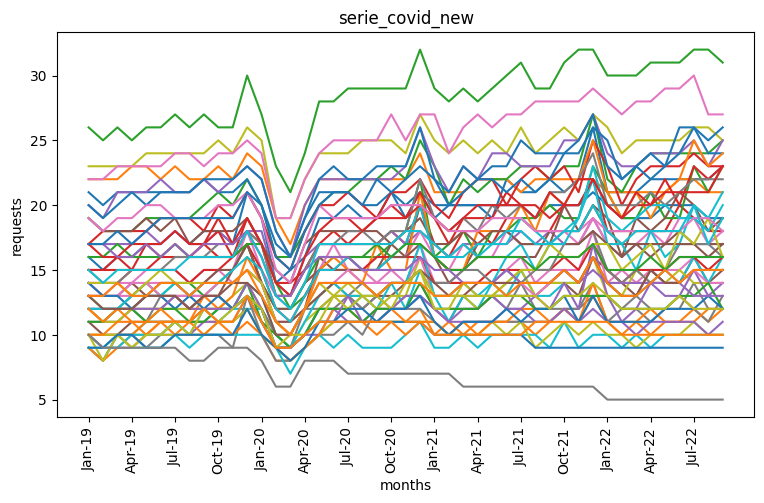
\includegraphics[width=0.5\textwidth]{serie_covid.png}%
%         \label{fig:covida}%
%         }%
%     \hfill%
%     \subfloat[Preprocessed data]{%
%         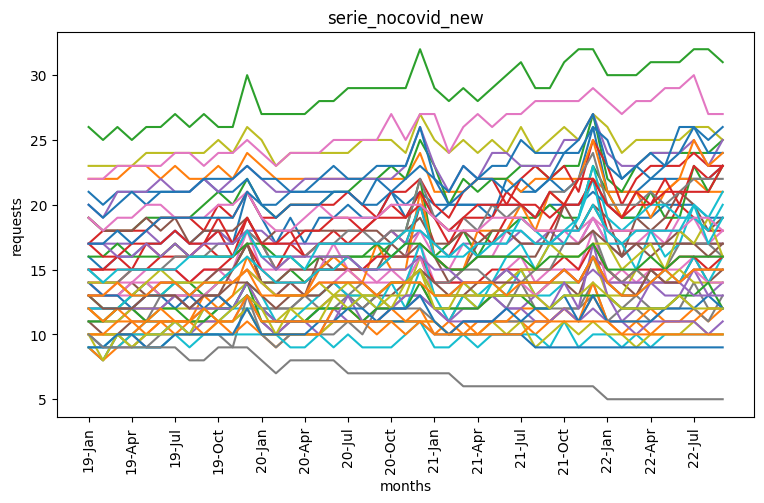
\includegraphics[width=0.5\textwidth]{serie_nocovid.png}%
%         \label{fig:covidb}%
%         }%
%     \caption{Input data.} % Main caption
%     \label{fig:test4}
% \end{figure*}

\section{The predictive module} \label{Sec:forecasting}

In our proposal, we utilize the Maximum Entropy Bootstrap (MEB) methodology in conjunction with the ensemble learning technique known as bagging (Bootstrap Aggregating). This combination enhances the accuracy and robustness of predictive models through the generation of multiple bootstrapped datasets from the original data. By training individual models on these datasets and aggregating their predictions through averaging, we adhere to MEB's principles while capturing the underlying statistical variability. Maximizing entropy under empirical constraints allows the integration of bagging with MEB to produce more robust models. In more details, each model trained on distinct bootstrapped samples incorporates uncertainty characteristics from the original data, allowing for a comprehensive representation of its variation.

The incorporation of MEB into the bagging framework not only bolsters the performance of predictive models but also facilitates uncertainty quantification in the predictions. Each model produces a set of predictions that can be used to construct confidence intervals, thereby offering insights into the variability and reliability of the forecasted outcomes. The ability to assess the spread of predictions from multiple bootstrapped datasets presents a more nuanced understanding of potential prediction intervals, which is particularly valuable in the context of the present paper, characterized by short, non-stationary, and possibly non linear time series surrounded by a significant amount of uncertainty.

Furthermore, this synergistic approach allows for dealing with noisy datasets and mitigating overfitting, as bagging inherently provides a mechanism to increase the robustness of the predictive model by leveraging the diversity across the bootstrapped samples. Since MEB generates bootstrapped datasets based on the maximum entropy principle, the resulting models avoid being overly sensitive to any one particular realization of the data.

Mathematically, if we denote the bootstrapped replicas of the dataset as $D^*_1, D^*_2, \ldots, D^*_B$, where $B$  represents the number of bootstrapped samples, the resulting predictive framework can be expressed as:  $\hat{y}_{\textit{BAG}} = \rho( \hat{y}_{b}(x) )$, where $\hat{y}_{b}(x)$ is the prediction made by the $b-th$ model trained on the bootstrapped sample $ D^*_b $  and $\rho$ a generic centrality parameter. 
This averaging process effectively reduces variance by smoothing out the predictions of the individual models, leading to enhanced stability and generalization capabilities in the final aggregated model.  The parameter $\rho$ is often defined as either a simple average or the median, which leads to the following bagging predictors:

\begin{equation}
\hat{y}_{\textit{BAG}}  = \frac{1}{B} \sum_{b=1}^{B} \hat{y}_{b}(x)
\end{equation}

\begin{equation}
\hat{y}_{\textit{BAG}}  = 
\begin{cases} 
\hat{y}_{b}(x) \left[\frac{h+1}{2}\right] & \text{if } h \text{ is odd} \\ 
\frac{\hat{y}_{b}(x)\left[\frac{h}{2}\right] + \hat{y}_{b}(x)\left[\frac{h}{2} + 1\right]}{2} & \text{if } h \text{ is even} 
\end{cases}
\end{equation}

here, $\hat{y}_{b}(x)$  is  sorted in ascending order whereas $h$ is the number of future values to be predicted.

\subsection{Resampling techniques} \label{Subsec:resampling}

%In recent years, resampling techniques, particularly the bootstrap method, have gained prominence as valuable tools for mitigating the inherent limitations of conventional forecasting approaches \citep{hasni2019spare}.  The bootstrap method, a non-parametric procedure, generates multiple simulated time series through resampling with replacement from the observed data. This methodology proves particularly advantageous when confronting the complexities of non-stationary, non-linear, intermittent and asymmetric cyclical patterns as well as scenarios characterized by a low signal-to-noise ratio \citep{chandran2024strategic,feliu2024enhancing,suman2024deep,zhang2024forecasting,kreiss2012bootstrap}.  Furthermore, resampling methods offer considerable utility in mitigating the effects of limited sample sizes \citep{dominguez2022machine} and in addressing model uncertainty \citep{sarris2020exploiting}. This provides logistics organizations with a more nuanced understanding of forecast uncertainty, enabling more precise risk management strategies and facilitating the adoption of more confident, data-driven decision-making processes \citep{ferrari2018bootstrap}.  The utility of bootstrap methods in statistical model selection has been extensively demonstrated through various studies. Fenga and Politis \citep{fenga2011bootstrap} introduced a bootstrap-based approach for autoregressive moving average (ARMA) order selection, showcasing its effectiveness in enhancing model accuracy and reliability in the presence of finite sample sizes. Their subsequent work \citep{fenga2013bootstrap} extended this methodology to threshold autoregressive models (SETAR), further validating bootstrap techniques as a robust mechanism for determining optimal model specifications. Moreover, Fenga and Politis \citep{fenga2017lasso} explored the application of the LASSO technique for sparse autoregression, underscoring a bootstrap framework that effectively addresses model selection in high-dimensional contexts. Collectively, these studies highlight how bootstrap methods can significantly improve order selection processes across various statistical modeling frameworks, demonstrating their broader applicability and relevance in contemporary statistical analysis.

%CAPOVERSO CHE COMINCIA DA RIGA 139 è SOSTITUITA DA QUESTO CHE SEGUE. \citep{dominguez2022machine} è stata sostiuita da  davison1997bootstrap che è piu' breve

In recent years, resampling techniques, especially the bootstrap method, have become valuable for overcoming the limitations of conventional forecasting methods \citep{hasni2019spare}. The bootstrap method creates simulated time series through resampling from observed data. This approach is useful for non-stationary, non-linear, intermittent, and asymmetric cyclical patterns, as well as low signal-to-noise scenarios \citep{feliu2024enhancing, suman2024deep, kreiss2012bootstrap}. Moreover, resampling methods help address the effects of limited sample sizes \citep{davison1997bootstrap}  and model uncertainty \citep{sarris2020exploiting}. 

The utility of bootstrap methods in model selection has been extensively validated. Fenga and Politis \citep{fenga2011bootstrap} introduced a bootstrap-based approach for autoregressive moving average (ARMA) order selection, demonstrating its effectiveness in enhancing model accuracy with finite sample sizes. Their work \citep{fenga2013bootstrap} extended this to threshold autoregressive models (SETAR), validating bootstrap techniques for optimal model specifications. Furthermore, Fenga and Politis \citep{fenga2017lasso} explored the LASSO technique for sparse autoregression, illustrating a bootstrap framework for model selection in high-dimensional contexts. These studies collectively show how bootstrap methods can enhance order selection across statistical modeling frameworks, underscoring their relevance in modern statistical analysis.

%The resampling scheme adopted here is called Maximum Entropy Bootstrap (MEB) \citep{meb1}. As it will be explained, MEB offers a principled and flexible approach to bootstrapping time series data, addressing many of the limitations of traditional block bootstrap methods. Its ability to handle complex dependencies and non-stationarity, coupled with its robust performance, makes it a valuable tool for a wide range of time series analysis tasks This powerful nonparametric resampling technique has revolutionized time series analysis by offering a principled and elegant approach to constructing bootstrap distributions \citep{meb2,meb3}. Unlike traditional block bootstrap methods (see, e.g., \citep{bb1,bb2}), which resample blocks of data to preserve the serial correlation structure, MEB seeks to maximize the entropy of the bootstrap distribution subject to constraints derived from the observed data. This approach leads to more flexible and less restrictive bootstrap distributions, offering several advantages over traditional methods, especially when dealing with complex time series data. A critical aspect of MEB’s application is its robustness in nonstationary environments, where traditional forecasting methods often falter. MEB can capture the evolving dynamics of the time series, thereby enhancing the predictive accuracy of the forecasts \citep{chen2020}. By generating multiple bootstrap samples, MEB facilitates the construction of confidence intervals and prediction intervals, which are paramount for effective decision-making in fields like finance and risk management \citep{shafer2019}. Furthermore, MEB allows for the incorporation of complex models, such as those involving seasonal patterns or autoregressive structures, into the resampling framework. This flexibility enables researchers to model intricate temporal dynamics, making MEB particularly suitable for various applications ranging from economic forecasting to climate modeling. Its capacity to integrate both linear and nonlinear dependencies provides a significant advantage over traditional methods that may oversimplify these relationships \citep{lopez2023}.

%CAPOVERSO CHE COMINCIA DA RIGA 146 è SOSTITUITO DA QUESTO CHE SEGUE

The standard bootstrap assumes independent and identically distributed (i.i.d.) data — an assumption that fails for time series, where observations are dependent and ordered.

This failure is more pronounced when the series is short, making dependence patterns more influential, the data exhibits autocorrelation, seasonality, or trend and when resampling destroys the structure and underrepresents variability.

In these cases Maximum Entropy Bootstrap (MEB) guarantees the following advantages:

\begin{itemize}
    \item {\it Preservetion of Dependence Structure } MEB maintains the temporal dependence (e.g., autocorrelation, trend, seasonality) by using rank-based and interpolation techniques that reorder and smooth the data. Unlike i.i.d. bootstrap, it doesn’t break time series structure.

    \item {\it Better Handling of Short Time Series } In short samples, structural properties (e.g., local trends) are easily lost by standard resampling. MEB keeps these features by reconstructing plausible time series paths that are consistent with observed data and uncertainty.

    \item {\it No Need for Model Specification} Unlike block bootstrap or parametric resampling, MEB is nonparametric and doesn’t require selecting block sizes or fitting ARMA models — a key benefit for short samples where such models may be unstable or overfitted.

    \item {\it Generation of Smooth Pseudo-Series} MEB produces continuous, smoothed pseudo-series through linear interpolation, making it well-suited for statistical inference tasks like forecasting, confidence intervals, and hypothesis testing.

    \item {\it Maximum Entropy Principle} It applies the maximum entropy principle, meaning the generated bootstraps are the least biased (i.e., most non-committal) estimates consistent with the known constraints (the observed data). This is especially valuable when little information is available — like in short series.

    \item {\it Support of Stationary and Non-Stationary Series} MEB is flexible with both stationary and non-stationary time series, whereas other bootstrap techniques often require stationarity or explicit transformation to achieve it.
\end{itemize}

The resampling scheme adopted here is called Maximum Entropy Bootstrap (MEB) \citep{meb1}. MEB offers a principled and flexible approach to bootstrapping time series data, leveraging the Maximum Entropy Principle (MEP) \citep{shannon1948mathematical} to address the inherent limitations of conventional bootstrap methods, thus addressing many limitations of traditional block bootstrap methods. The essence of MEP is grounded in the idea that in the absence of specific information, the most rational probability distribution to adopt is one that maximizes entropy, reflecting the greatest uncertainty about the system \citep{jaynes1957information}. This is mathematically articulated through Shannon entropy,  defined as $S(p) = -\sum_{i=1}^{n} p_i \log(p_i)$, where $ p_i$ denotes the probability associated with the i-th outcome within a discrete sample space of size $n$. 
% Its ability to handle complex dependencies and non-stationarity, along with robust performance, makes it valuable for a wide range of time series analysis tasks. This powerful nonparametric resampling technique has transformed time series analysis by providing an elegant method for constructing bootstrap distributions \citep{meb2, meb3}. 

% Unlike traditional block bootstrap methods \citep{bb1, bb2}, which resample data blocks to preserve serial correlation, MEB maximizes the entropy of the bootstrap distribution subject to constraints from the observed data. This results in more flexible bootstrap distributions, offering advantages over traditional methods, especially for complex time series data. A critical aspect of MEB is its robustness in nonstationary environments, where traditional forecasting methods may struggle. MEB captures evolving time series dynamics, enhancing forecast accuracy \citep{chen2020}. By generating multiple bootstrap samples, MEB facilitates the construction of confidence and prediction intervals, crucial for effective decision-making in finance and risk management \citep{shafer2019}. Furthermore, MEB accommodates complex models involving seasonal patterns or autoregressive structures, enabling researchers to model intricate temporal dynamics. Its ability to integrate linear and nonlinear dependencies provides a significant advantage over traditional methods that may oversimplify relationships \citep{lopez2023}.

% The Maximum Entropy Bootstrap (MEB) \citep{Vinod1993,Vinod2006,Kourentzes2015,Vinod2008} represents a systematic approach to resampling that integrates the principles of information theory with statistical inference, leveraging the Maximum Entropy Principle (MEP) \citep{shannon1948mathematical} to address the inherent limitations of conventional bootstrap methods. The applications of MEB extend across various disciplines such as econometrics, ecology, and social sciences, wherein empirical data often suffer from limitations such as small sample sizes or biased distributions. The flexibility of MEB allows researchers to incorporate prior knowledge through constraints while maximizing uncertainty and ensuring that the bootstrap samples reflect a realistic representation of the original dataset. MEB offers a compelling alternative to traditional bootstrap methodologies—especially in scenarios where the underlying distribution is unknown or when the sample data is not sufficiently large to assume a normal distribution. The essence of MEP is grounded in the idea that in the absence of specific information, the most rational probability distribution to adopt is one that maximizes entropy, reflecting the greatest uncertainty about the system \citep{jaynes1957information}. This is mathematically articulated through Shannon entropy,  defined as $S(p) = -\sum_{i=1}^{n} p_i \log(p_i)$, where $ p_i$ denotes the probability associated with the i-th outcome within a discrete sample space of size $n$. 

The pivotal advancement provided by MEB lies in its ability to formulate bootstrapped samples that adhere to a spectrum of constraints dictated by the original dataset, such as predetermined moments, probabilities, or other statistical characteristics \citep{berger1985statistical}. Specifically, under typical circumstances, these constraints can be specified in the form of normalized probabilities and empirical expectations, expressed as $\sum_{i=1}^{n} p_i = 1$ to ensure that the probabilities form a valid distribution, and $\sum_{i=1}^{n} p_i f_i = \bar{f}$, where $f_i$ represents measurements or statistics relevant to the analysis, with $\bar{f}$ being the empirical mean of these measurements. The formulation of the Maximum Entropy problem consequently leads to a constrained optimization framework. The optimization problem can be succinctly encapsulated in the Lagrangian: $ L(p, \lambda, \mu) = S(p) + \lambda \left(1 - \sum_{i=1}^{n} p_i\right) + \mu \left(\bar{f} - \sum_{i=1}^{n} p_i f_i\right)$, where $\lambda$ and $\mu$ are Lagrange multipliers that adjust the balance under the constraints of normalizing the distribution and matching the empirical mean, respectively. The solution to this maximization problem yields a probability distribution, which appears as $p_i = \frac{e^{\mu f_i}}{\sum_{j=1}^{n} e^{\mu f_j}}$, where the parameter $\mu$ is determined through the constraint equations, specifically via a numerical root-finding approach that satisfies the moment condition $\sum_{i=1}^{n} p_i f_i = \bar{f}$.

This formulation transforms the problem into one that allows for flexible adaptation to various types of data and constraints imposed by the empirical observations. Once this maximum entropy distribution is established, resampling via bootstrapping can commence by selecting  $m$ samples according to the derived $ p_i$.  This produces synthetic datasets that not only reflect the variability and uncertainty characteristic of the original data but also adhere to the specific constraints imposed, which may include higher moments or even domain-specific statistics. 

This resampling process can be iterated to generate a comprehensive set of bootstrapped samples, enabling a multitude of statistical analyses, including confidence interval estimation, hypothesis testing, and model validation \citep{efron1993introduction}. We adopted this procedure to generate the bootstrap sets of dataseries upon which scenarios were defined as detailed in the following section.

%%%%%%%%%%%%%%%%%%%%%%%%%%%%%%%%%%%%%%%%%%%%%%%%%%%%%%%%%%%%%%%%%%%%%%%%%%%%%%
\section{The prescriptive module} \label{Sec:optimization}

The results of the predictive module are the input to the prescriptive module, whose goal is to optimize the allocation of stores to DCs. The result of the optimization is used to evaluate the modeled {\it scenario}, where scenarios are defined for specific what-if analyses. For example, the objective of the what-if analyses could be the effect of freezing some allocations while leaving the rest free, or possibly accepting some multiple, in our test case double, allocations for some selected stores. 

The core optimization problem is a split allocation problem. This variant of the basic allocation problem has already received attention in the optimization literature, mainly in the context of survivable communication network design \citep{EK98,MKE75}, and more generally as the splittable capacitated multiple allocation hub location problems \citep{M05}, and finds applications in fiber optic access networks \citep{KLH11}, split delivery routing \citep{DT89}, and even in school timetabling \citep{BBL07}. A problem closely related to the one of interest to us is presented in \citep{ZHHY21}.

The mathematical model we use is a direct extension of the standard model for the allocation problem. Since the framework we propose has validity beyond the specific case study described in the paper, in the following, we will refer to the actual application elements (stores and DCs) by a more standard allocation nomenclature, using the terms {\it clients} for stores and {\it servers} for DCs interchangeably. In our case, assignment constraints can accept up to a parametric number of assignments, allowing the service of requests to be distributed across multiple servers. The notation used in the model is as follows:

\begin{enumerate}
    \item[$n$] number of clients (stores)
    \item[J] index set of clients, $J=\{1, \ldots, n\}$
    \item[$m$] number of servers (DCs)
    \item[I] index set of servers, $I=\{1, \ldots, m\}$
    \item[$c_{ij}$] global cost for allocating client $j \in J$ to server $i \in I$
    \item[$Q_i$] storage capacity of server $i \in I$
    \item[$d_i$] unit storage cost of server $i \in I$
    \item[$req_j$] total request of client $j$.
    \item[$b_j$] maximum number of servers (DCs) client $j$ can be assigned to
    \item[$x_{ij}$] binary decision variable equal to 1 iff client $j$ is allocated to server $i$, $i \in I$ and $j \in J$
    \item[$q_{ij}$] integer decision variable representing the amount (number of pallets) of request of client $j$ provided from server $i$
\end{enumerate}

In the final test case, the amount requested by each client was always set to be equal to the corresponding predicted value, but in some scenarios, the requests of some clients could be explicitly split between two servers, so the requested $q_{ij}$ amounts could vary.

The mathematical model used for this problem was as in the following formulation FD.
   
\begin{align}
&(FD) & z_{FD} = \textbf{min } & \sum_{i \in I} \sum_{j \in J} ( c_{ij}x_{ij} + d_i q_{ij} ) \label{ALLobj}\\
& &  \textbf{subject to }
     & \sum_{i \in I} q_{ij} = req_j & j \in J  \label{ALLrequest}\\
& &  & \sum_{j \in J}q_{ij} \leq Q_i & i \in I \label{ALLcapacity}\\
& &  & \sum_{i \in I} x_{ij} = b_j & j \in J  \label{ALLnumserv}\\
& &  & q_{ij} \leq req_j x_{ij} & i \in I, j \in J \label{ALLcontin}\\
& &  & x_{ij} \in \{0,1\} & i\in I, j \in J \label{ALLx}\\
& &  & q_{ij} \in \mathbb{Z}^+_0 & i\in I, j \in J \label{ALLq}
\end{align}

Constraints \ref{ALLnumserv} are formulated as equalities because of the need to impose specific splits in what-if settings. If this is not of particular interest, these constraints could be replaced by less-than-or-equal-to inequalities combined with inequalities that force allocations to at least one server.

Note that when $b_j = 1$ for all clients, i.e., when each client $j \in J$ can be served by only one server, constraints \ref{ALLcontin} and \ref{ALLrequest} force the entire quantity requested by client $j$, $req_j$, to be supplied by a single server. The constraints \ref{ALLcontin} thus become equations, the constraints \ref{ALLrequest} become redundant, and the constraints \ref{ALLcapacity} can be expressed by replacing $\sum_{j \in J}q_{ij}$ with $\sum_{j \in J}req_j x_{ij}$. Problem P reduces to the standard GAP and can be solved by any of the methods described in \citep{matheuristics}.

However, we are interested in the general case that allows some multiple assignments, and since the cost is derived from the assignments, the problem can be considered a fixed-cost, split-assignment allocation problem.

Moreover, since future client requests can only be forecast, the problem can be more conveniently formulated as a stochastic optimization problem \citep{KM10,BL11}, where future requests are random variables $\rho_j$, $j \in J$, whose distributions can be derived from the forecast results. The problem becomes a single-stage stochastic problem, since there is no subsequent recourse, whose formulation is as follows.

\begin{align}
&(FS) & z_{FS} = \textbf{min } & \sum_{i \in I} \sum_{j \in J} ( c_{ij}x_{ij} + d_i q_{ij} ) \label{SALLobj}\\
& &  \textbf{subject to }
     & \sum_{i \in I} q_{ij} = R(\rho_j) & j \in J  \label{SALLrequest}\\
& &  & \sum_{j \in J}q_{ij} \leq Q_i & i \in I \label{SALLcapacity}\\
& &  & \sum_{i \in I} x_{ij} = b_j & j \in J  \label{SALLnumserv}\\
& &  & q_{ij} \leq R(\rho_j) x_{ij} & i \in I, j \in J \label{SALLcontin}\\
& &  & x_{ij} \in \{0,1\} & i\in I, j \in J \label{SALLx}\\
& &  & q_{ij} \in \mathbb{Z}^+_0 & i\in I, j \in J \label{SALLq}
\end{align}

\noindent where the values $R(\rho_j)$ in the constraints \ref{SALLrequest} and \ref{SALLcontin} refer to any same realization of the random variable $\rho_j$.

Different methods can be used to deal with this case \citep{SDR09}. We transformed the formulation (FS) into its {\it deterministic equivalent} \citep{D55} using the forecasts computed on the bootstrap sets. This transformed the original stochastic problem into a deterministic optimization one. We generated multiple scenarios each containing a realization of the stochastic variable $\rho$, which is defined as a forecast of one series from the bootstrap set in use. For each scenario $s$, we thus created a version of the constraint with $b_i^{s}$ as the right-hand side. The final solution must satisfy these constraints across all scenarios.

The objective function now incorporates the various quantities that must be delivered to each client in different scenarios. We therefore consider the expected cost as a weighted average across the scenarios and include it in the objective function. 

The resulting formulation is as follows. The random variables $\rho_j$ are sampled in a finite number of scenarios. Let $\rho^s_j$ denote the realization of $\rho_j$ in scenario $s$, $s \in S$, and let $p_s = \frac{1}{|S|}$ be the probability associated with scenario $s \in S$. The variables $\epsilon_{js}$ are slack variables for the customer service constraints.

\begin{align}
&(DE) & z_{DE} = \textbf{min } & \sum_{s \in S} \left( p_s \sum_{j \in J} \left( \sum_{i \in I} ( c_{ij}x_{ij} + d_i q_{ij}^s) + M \epsilon_{js} \right) \right) \label{DEobj}\\
& &  \textbf{subject to }
     & \sum_{i \in I} q_{ij}^s + \epsilon_{js} = \rho_j^s & j \in J, s \in S \label{DErequest}\\
& &  & \sum_{j \in J}q_{ij}^s \leq Q_i & i \in I, s \in S \label{DEcapacity}\\
& &  & \sum_{i \in I} x_{ij} = b_j & j \in J  \label{DEnumserv}\\
& &  & q_{ij}^s \leq \rho_j^s x_{ij} & i \in I, j \in J, s \in S \label{DEcontin}\\
& &  & x_{ij} \in \{0,1\} & i\in I, j \in J \label{DEx}\\
& &  & q_{ij}^s \in \mathbb{Z}^+_0 & i\in I, j \in J, s \in S \label{DEq}\\
& &  & \epsilon_{js} \in \mathbb{Z}^+_0 & j \in J, s \in S \label{DEeps}
\end{align}

In this formulation, since each variable $\rho_j^s$ corresponds to a specific realization of the corresponding random variable $\rho_j$, the amounts to be delivered to each store $j \in J$ are scenario-specific. However, it is required to determine a unique allocation that allows to serve all stores in any proposed scenario. This last requirement may be infeasible, so the slack variables $\epsilon_{js}$ are needed in the formulation. They are lexicographically penalized in the objective function by appropriately high costs, in order to implement the primary concern of achieving feasibility.

Optimizing formulation (DE) makes it possible to determine the quantities that each server must be able to supply to each client, i.e. the total quantity that each server must handle. 

In terms of our logistical application, since each DC must maintain sufficient inventory to meet the anticipated demand during the designated period, the optimization of the client (retailer) allocation translates directly into a quantification of the DC inventory and therefore of its required minimum size. The solution of the allocation problems permits therefore to directly solve the dimensioning question that motivated this research.

\section{Computational results} \label{Sec:results}

The two modules, predictive and prescriptive, are run in sequence, the first generating input to the second. This section reports the results obtained for the validation of each of them, when implemented according to the specifications previously described.

\subsection{Predictive module tests} \label{Subsec:predictive}

The objective of the predictive module is to forecast the demand for each of the stores considered,  asking for a forecast three months ahead.

The available data consists of a time series for each of the 52 stores considered. Each series contains 45 values, corresponding to 4 years of monthly data of relevant requests for each store, minus the values for the last 3 months to be forecast.

The core approach put forth in this paper is the bootstrap method described in section \ref{Sec:forecasting}. These results are validated against those obtained by means of several alternative forecasting algorithms, namely SARIMAX, Holt-Winters, MLP, RNN (LSTM), random forest and gradient boosting (XGboost). For each of these algorithms, the relevant hyperparameters were determined by grid search when they were all integer-valued, such as in the case of SARIMAX, and by Hammersley sampling \citep{H60} when real valued parameters were involved. 

All series were pre-processed with a log-diff transform to approach stationarity and with a max-min scaler for the artificial intelligence derived methods. The implementation language was python, version 3.11, in all cases and the codes were run on a Windows PC workstation equipped with four Intel Core i7-4790 CPUs running at 3.60GHz and 32 GB of RAM.

The focus of this part of the research is on the bootstrap method. To this end, we tested the approach with the following settings:
\begin{itemize}
\item bootstrap sets containing 75, 125 and 175 series;
\item bootstrap sets generated by simple autoregressive AR(p) with p=5 model (the default in python's statsmodels), where parameters are estimated using Yule-Walker equations \citep{BD91}, and by ARIMA, where autoarima is run on each of the seed series and the optimized orders are then applied to each boosted series;
\item the forecasting of all the boosted series generated as above to obtain the boosted forecasts was tested with AR(p), Random Forest or ARIMA. In the case of ARIMA, autoarima was only repeated on the first series of each bootstrap set. In the case of AR, the parameter p was set for each series after a loop on different p values, keeping the one that maximised the corresponding AIC value.
\end{itemize}

We also tried to generate the bootstrap sets with and without backcasting and with simple extraction with repetitions among the residuals of the seed series and with their scrambling. The results of these tests are not reported because backcasting induces a worsening of the results, while scrambling the residuals shows no difference with respect to the extraction with repetitions, so we decided to use the latter in line with the literature.

Forecasts were compared using 3 cost functions, Mean Absolute Error (MAE), Mean Square Error (MSE), and Bias. The results are obtained by ranking the corresponding forecasts for each series according to the quality of the function considered, as we want to emphasize how the algorithms perform relative to each other, and then averaging each function rank over all series. Absolute values for the error measures, not rank-based, are reported for all boostset sizes in the appendix \ref{app:errcost}. Table \ref{table:YWARranks} presents results where the forecasts obtained with the standard algorithms are compared with the forecasts obtained by boosting, where the boosted series were computed by an AR(5) model based on the Yule Walker equations, the forecast of these series was then obtained by a simple autoregressive model, and the boosted sets consisted of 75 series (columns under heading $YW\_AR\_75$), 125 series (heading $YW\_AR\_125$), and 175 series (heading $YW\_AR\_75$).

The columns show the average ranking of each cost function (MAE, MSE or bias) for each boostset size, while on the rows we report:

\begin{itemize}
  \item $fcast\_avg$: boost forecast obtained as the average of the corresponding ranks;
  \item $fcast\_50$: boost forecast obtained as the median of the corresponding ranks;
  \item $yar$: non-boost forecast obtained by an AR model;
  \item $yarima$: non-boost forecast obtained by an ARIMA model;
  \item $yhw$: non-boost forecast obtained by a Holt and Winters model;
  \item $ymlp$: non-boost forecast obtained by a multilayer perceptron model;
  \item $ysvm$: non-boost forecast obtained by a SVM model;
  \item $ylstm$: non-boost forecast obtained by a LSTM model;
  \item $yrf$: non-boost forecast obtained by a random forest model;
  \item $yxgb$: non-boost forecast obtained by a XGboost model;
\end{itemize}

\vspace{0.3cm}
\begin{table}
\centering
\renewcommand{\arraystretch}{0.75}
\begin{tabularx}{\textwidth}{l|CCC|CCC|CCC}
 & \multicolumn{3}{|c|}{YW\_AR\_75} &  \multicolumn{3}{|c|}{YW\_AR\_125}  &  \multicolumn{3}{|c}{YW\_AR\_175} \\
 & MAE & MSE & bias & MAE & MSE & bias & MAE & MSE & bias \\
\hline
fcast\_avg& 2.67 & 2.67 & 0.08 & 2.58 & 2.58 & 0.05 & 3.83 & 3.83 & 0.04 \\
fcast\_50 & 3.04 & 3.04 & 0.06 & 3.19 & 3.19 & 0.04 & 2.50 & 2.50 & 0.03 \\
yhw       & 5.42 & 5.42 & 0.08 & 6.06 & 6.06 & 0.04 & 5.88 & 5.88 & 0.03 \\
yarima    & 5.73 & 5.73 & 0.05 & 6.04 & 6.04 & 0.03 & 6.08 & 6.08 & 0.02 \\
ysvm      & 5.88 & 5.88 & 0.08 & 5.50 & 5.50 & 0.05 & 5.50 & 5.50 & 0.03 \\
ylstm     & 6.02 & 6.02 & 0.06 & 5.52 & 5.52 & 0.04 & 6.27 & 6.27 & 0.02 \\
yar       & 6.06 & 6.06 & 0.04 & 6.54 & 6.54 & 0.02 & 6.79 & 6.79 & 0.02 \\
ymlp      & 6.38 & 6.38 & 0.05 & 5.98 & 5.98 & 0.03 & 6.17 & 6.17 & 0.02 \\
yrf       & 6.46 & 6.46 & 0.11 & 6.31 & 6.31 & 0.06 & 5.48 & 5.48 & 0.04 \\
yxgb      & 7.33 & 7.33 & 0.12 & 7.29 & 7.29 & 0.07 & 6.50 & 6.50 & 0.05 \\
\hline
\end{tabularx}
\caption{Average rankings for different boostset size.}
\label{table:YWARranks}
\end{table}

The table shows that boosting is consistently the most reliable method for minimizing forecast errors, even when forecasts are obtained from a model as simple as AR[p], while ARIMA produces the least bias.

Figure \ref{fig:distr} shows two examples of forecast distributions obtained for two different series. The green bars correspond to the distribution of the results obtained by the AR[p] model over the differently recolored alternatives of a series. Lines representing the results of other forecasting algorithms applied to the original series are superimposed on the distribution.


\begin{figure}[ht]
\centering
\begin{minipage}{0.48\textwidth}
    \centering
    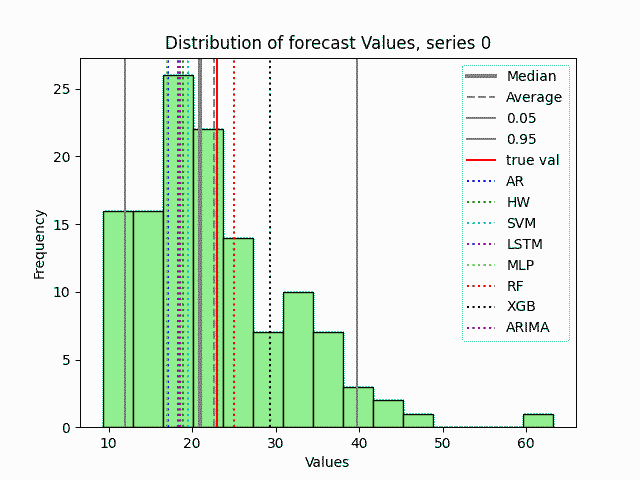
\includegraphics[width=\linewidth]{distr_75_0.png}
    \label{fig:dista}%
    \vspace{0.5em}
    \textit{(a) 75 bootset}
\end{minipage}
\hfill
\begin{minipage}{0.48\textwidth}
    \centering
    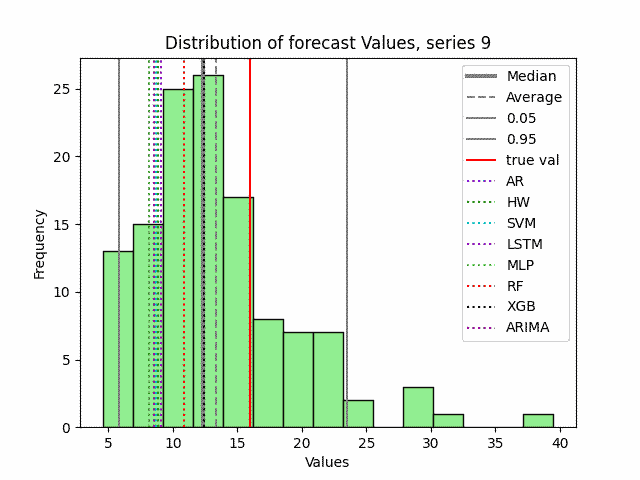
\includegraphics[width=\linewidth]{distr_75_9.png}
    \label{fig:distb}%
    \vspace{0.5em}
    \textit{(b) 125 boostset}
\end{minipage}
\caption{Distribution of bootstrap forecasts.}
\label{fig:distr}
\end{figure}

The relative merits of the different forecasting approaches are better highlighted by critical difference diagrams based on the non-parametric Friedman test followed by a post-hoc Nemenyi test. They allow for a visual comparison of performance ranks, and show whether differences between classifiers are statistically significant \citep{D06}. The graphs, generated in our case by their SciKit version \citep{SciKitCD}, plot the average rank across all series for each algorithm along the x-axis and connect by a horizontal bar those that could not be considered statistically different.

Figures \ref{fig:ywar75} and \ref{fig:ywar175} show a comparison of the ranks on MAE for the 75 series boostset and on MSE for the 175 series boostset. In both cases, as in all those tested, the accuracy of the boost forecasts is significantly higher than that obtained with alternative models. The tables in Appendix \ref{app:errcost} confirm that the comparison gives consistent results across all boostset sizes and cost functions, except for bias. The bias rankings are in fact unrelated to those obtained with the other cost functions, but this is due to the fact that the bias is very small in all cases, less than 1\% of the average of the empirical values, which ensures that all the forecasting models are free of systematic errors on our data and makes the difference in the rankings insignificant.

\begin{figure*}[ht] 
    \centering
    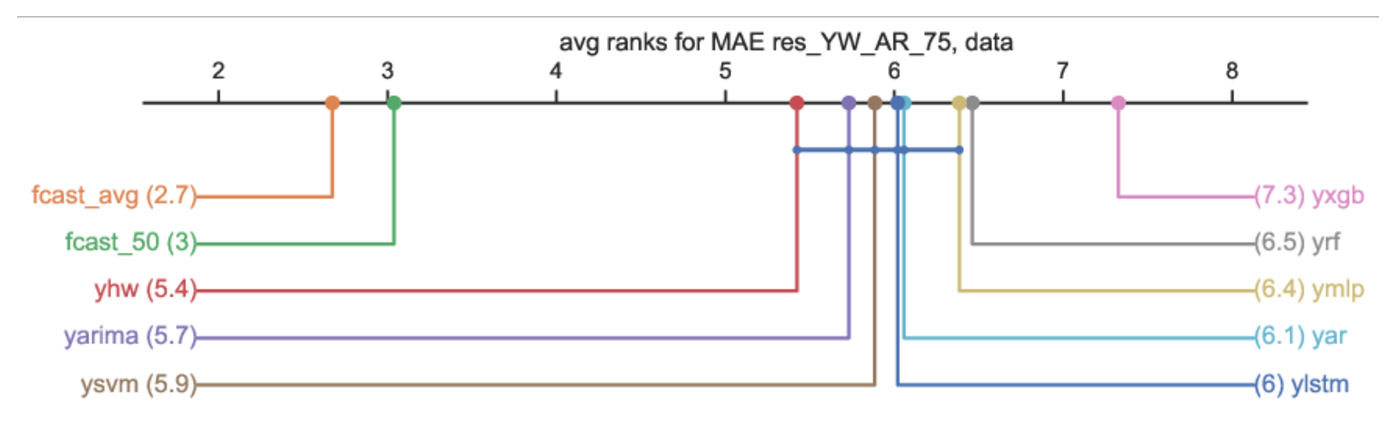
\includegraphics[width=0.75\linewidth]{sp_MAE_res_YW_AR_75.eps}%
    \caption{Average ranks for MAE on instance res\_YW\_AR\_75}
    \label{fig:ywar75}
\end{figure*}

\begin{figure*}[ht] 
    \centering
    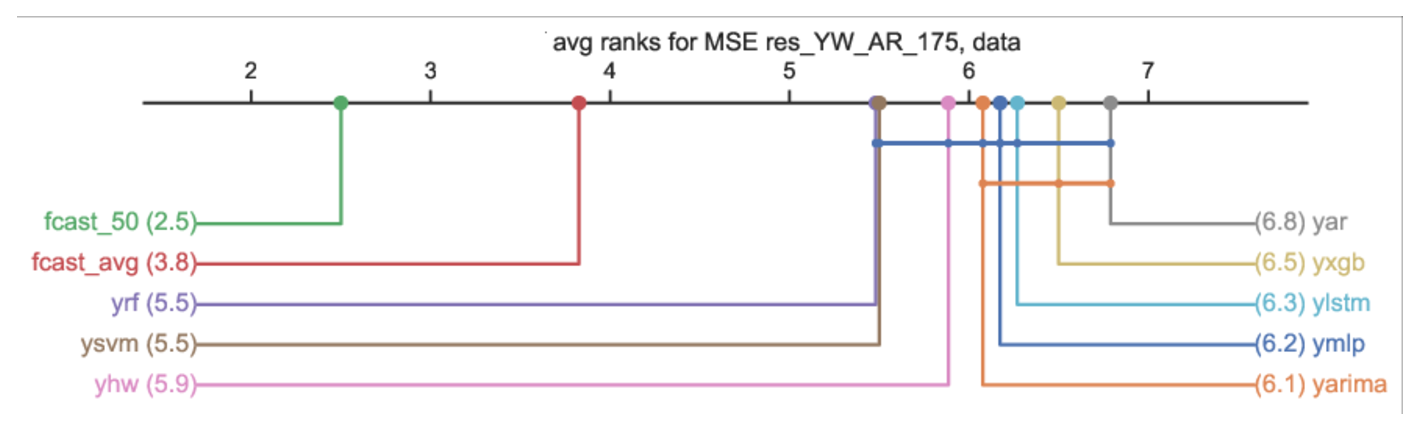
\includegraphics[width=0.75\linewidth]{sp_MSE_res_YW_AR_175.eps}%
    \caption{Average ranks for MSE on instance res\_YW\_AR\_175}
    \label{fig:ywar175}
\end{figure*}

These relatively short time series require a forecasting approach that is robust to both limited data and nonstationarity.  While sophisticated machine learning models such as Recurrent Neural Networks (RNNs) and Gradient Boosting Machines (GBMs) have gained prominence in recent years, their performance can be negatively affected by limited data availability, especially in cases with non-stationary properties, leading to potential overfitting.  The autoregressive (AR) model, combined with maximum entropy bootstrap, offers a powerful and promising alternative.  This technique demonstrates excellent performance in the context of this study, consistently outperforming more complex machine learning models, and offers an approach based on robust statistical principles that mitigates the risk of overfitting inherent in many AI approaches. The AR model, combined with the bootstrap methodology, moreover provides reliable forecasts that are ideally suited for integration into the subsequent optimization module.  

The choice of an autoregressive (AR) model, in addition to its better accuracy in our case, offers several crucial advantages over more complex machine learning approaches. First, the inherent simplicity of the AR model contributes to its ease of implementation and interpretation.  Unlike many machine learning algorithms that operate as "black boxes," the parameters of the AR model have clear statistical interpretations that provide insights into the underlying dynamics of the time series data. Second, the AR model's well-established theoretical framework and readily available diagnostic tools allow for robust validation and assessment of model performance.  

\subsection{Prescriptive module tests}  \label{Subsec:prescriptive}

The results reported in section \ref{Subsec:predictive} suggested instantiating the optimization on the results provided by the bootstrap forecasts. The prescriptive module was first run in a deterministic setting, to define a benchmark solution, then extended to the stochastic setting described in section \ref{Sec:optimization}.

When the problem to be solved is modeled as in the (FD) formulation, using the average predictions obtained by boosting as deterministic data, the instance is easily solved by any state-of-the-art MILP solver, thus ensuring the viability of dealing with a significant deterministic equivalent of the stochastic formulation (FS). The optimal deterministic value, $z_{FP}=$15553, is used as a benchmark in the following tests.

We moved on to the (DE) formulation generating $|S|=100$ scenarios by randomly sampling the stochastic variables $\rho_j$ over the associated probability distributions of the values resulting from the forecasts on all series that are part of a boostset. 
Given these input data, we ran experiments to assess the impact of the variation of the remaining sets of parameters of the formulation, i.e., cardinality of the boostsets, number of splittable clients, and assumptions on inventory costs. 

All reported tests were run on the same machine as in subsection \ref{Subsec:predictive}, a Windows PC workstation equipped with four Intel Core i7-4790 CPUs running at 3.60 GHz and 32 GB of RAM, but in this case the implementation language was C++ to allow finer control over the MILP solver used, which was CPLEX v. 22.11.

\subsubsection*{Increasing boostset size}

The size of the boostset helps to stabilize the results during forecasting, but it has a deep impact on the optimization. In fact, while the number of variables and the number of constraints of the formulation DE do not depend on the boostset size, larger boostsets are more likely to contain unusual values or combinations thereof, thus making constraints (\ref{DErequest}) progressively harder to satisfy, thus more costly, and possibly rendering the instance infeasible.

We conducted experiments to ascertain this using 75, 125 and 175 series boostsets and a 600 second time limit on the optimization process. Figure \ref{fig:bsize} shows a boxplot diagram depicting the distribution of the optimized cost over a number of tests equal to 1/5 of the number of series in the boostset, i.e., 15, 25, 35, respectively.

\begin{figure*}[ht] 
    \centering
    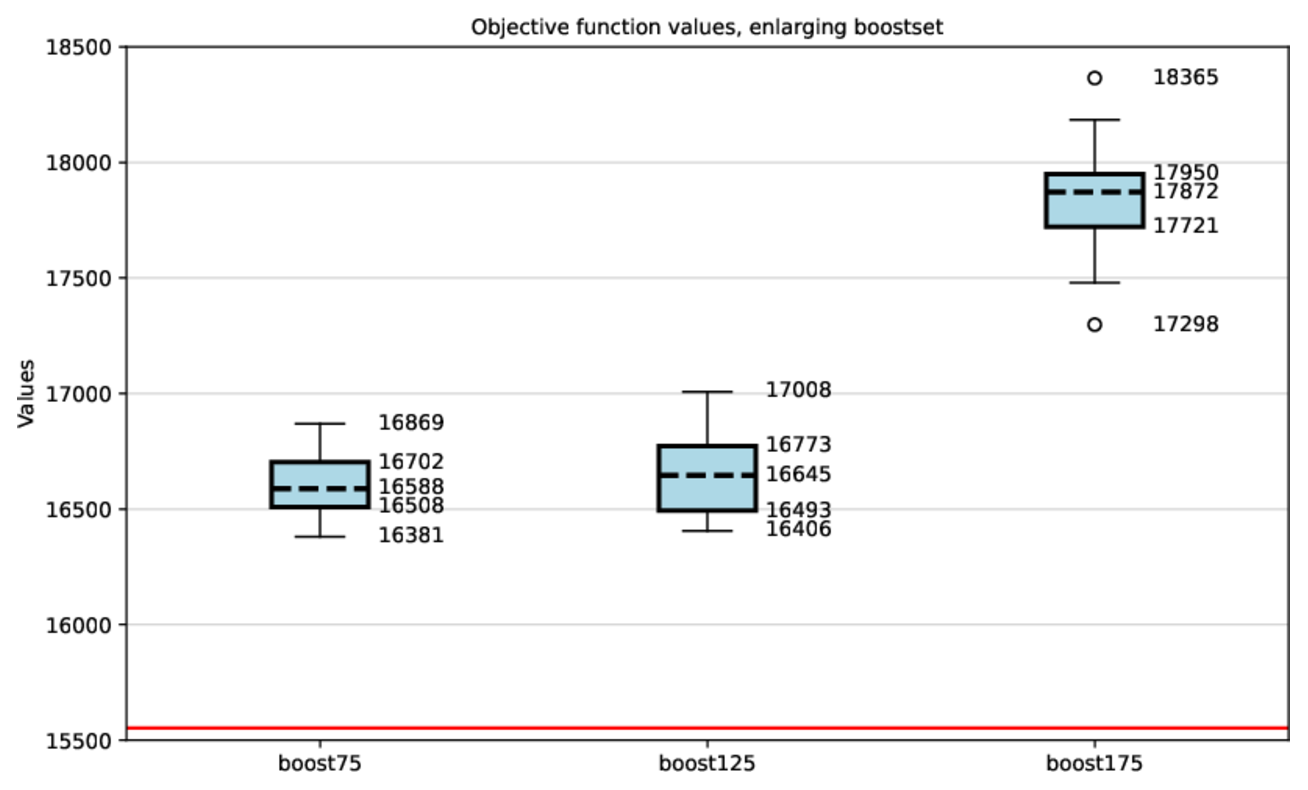
\includegraphics[width=0.7\linewidth]{figb0.eps}%
    \caption{Allocation cost for increasing boostset size}
    \label{fig:bsize}
\end{figure*}

Figure \ref{fig:bsize} has a red horizontal line at the value of the cost of the deterministic case. The increase in cost can therefore be considered as a quantification of the value of the information about the storage requests. We notice that the cost is essentially stable in the cases of the 75 and 125 series sets, but increases significantly in the case of the 175 boostset. This is due to the increased difficulty of the larger boostset instances, which leads to some instances being solved only heuristically within the time limit. All instances were feasible, but 7 out of 35 still had a gap between lower and upper bound after 600 seconds of CPU time. 

Finally, we note that if we take the optimal solution obtained with the coefficients imposed by the 75 series and evaluate it with the coefficients of the 125 series, we obtain (obviously) a more costly solution than the optimal one computed with the coefficients of the 125 series, but more interestingly, we have a solution that is not feasible with the coefficients of the 175 series.

\subsubsection*{Increasing number of splittable clients}

A defining feature of the problem we face is the possibility of accepting split service for some clients. This is unusual for allocation problems and results from the requirement to perform specific what-if analyses on the results. The number of clients allowed to split, and which ones they are, is given in input. In the actual case, the service to a client, if splittable, could be split between at most two servers, and the quantities delivered had to be integer, as specified in all formulations..

Obviously, the clients to split are chosen from the most requesting clients. We ran a series of tests based on 75 series boostsets, allowing the 0, 4, 8, and 12 most requesting clients to be split. Figure \ref{fig:bmult} shows the corresponding boxplots.

\begin{figure*}[ht] 
    \centering
    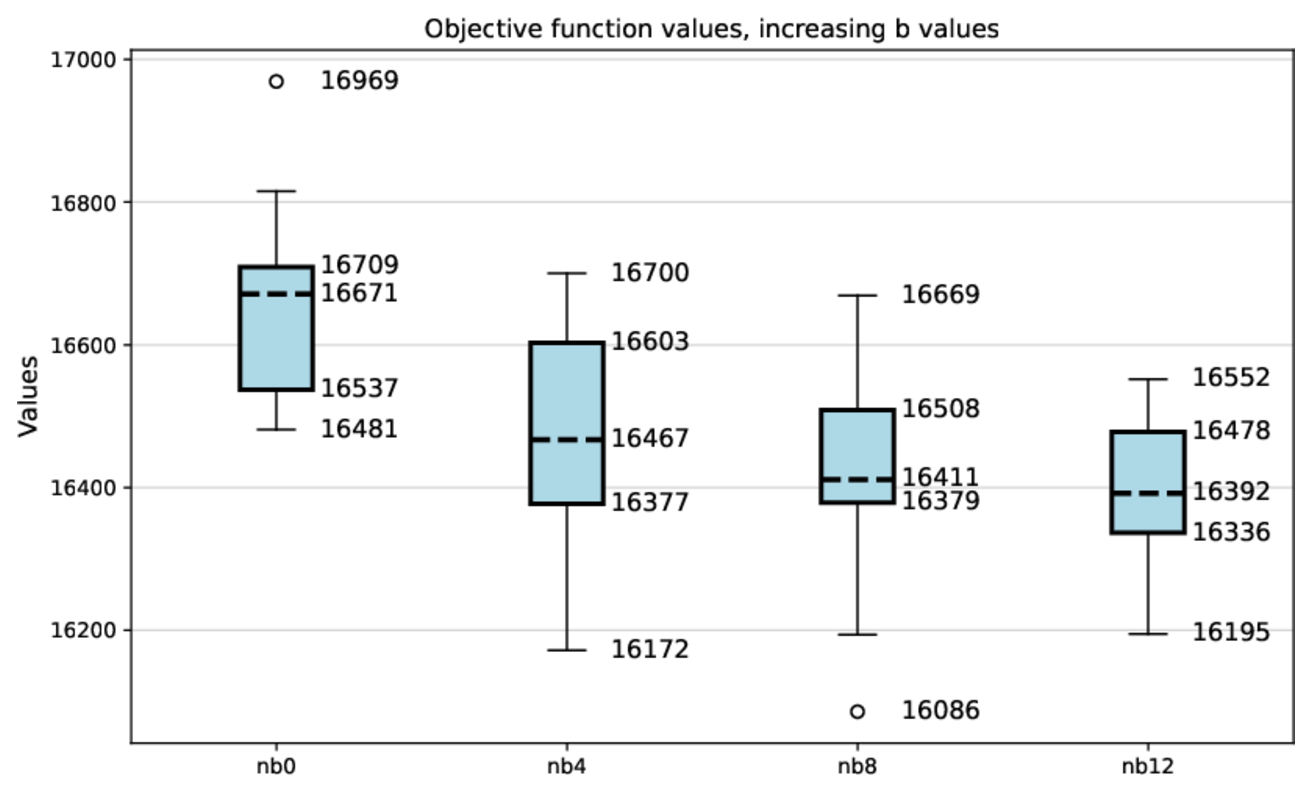
\includegraphics[width=0.7\linewidth]{figbmult.eps}%
    \caption{Allocation cost for increasing number of splittable clients}
    \label{fig:bmult}
\end{figure*}

Allowing the service to a client to be split is a partial relaxation of the corresponding assignment constraint, so the optimal cost is expected to decrease. Indeed, this can be seen in figure \ref{fig:bmult}, where the more clients are allowed to split, the lower all distribution moments are. However, the marginal decrease becomes smaller as the number of splittable clients increases, since splitting a small client may result in only a small contribution, if any.

\subsubsection*{Impact of different inventory cost assumptions}

A further set of tests was conducted to determine the impact of inventory costs $d_i$, $i \in I$ on the search process. Recall that in the original case study, one of the objectives was to determine how much space should be rented in the only DC not owned by the company, where storage space needs to be leased. The case study reported in \citep{MZ23} did not include storage costs. Here, we consider storage costs that are inversely proportional to the average distance of the DC from the stores. We consider three settings, one with no storage costs, one where only the most distant DC incurs costs, and one where all DCs need to lease space. Costs are proportional to the quantities stored and are therefore influenced by the allocation policy.

All tests were performed on the 75 series boostset. The interest of the analysis does not lie in the increase of the optimal costs, since an increase of the costs of the decision variables clearly leads to an increase of the global costs, but rather in the variation of the complexity of the search, as it is reflected in the CPU time to reach the final result, and in the optimality or feasibility of the solutions. To assess the effectiveness of increasingly longer searches, we report results after 600, 1200 and 3600 seconds of CPU time.

The results are summarized in the table \ref{table:qcost}. All results are based on 15 repetitions, and the columns show:

\begin{itemize}[noitemsep,nolistsep]
    \item $n$: number of clients (stores);
    \item $m$: number of servers (DCs);
    \item $n_{boost}$: number of series in the boostset;
    \item $n_q$: number of servers incurring leasing costs;
    \item $n_{inf}$: number of infeasible solutions at the end of the search;
    \item GAP lin: average gap between the linear bound and the best solution at the end of the search;
    \item GAP fin: average gap between the best lower bound and the best solution at the end of the search;
    \item t.CPU: average CPU time (in sec) of the search process.
\end{itemize}

\vspace{0.3cm}
\begin{table}
\centering
\renewcommand{\arraystretch}{0.75}
\begin{tabularx}{0.8\textwidth}{CCCC|CCCC}
$n$ & $m$ & $n_{boost}$ & $n_q$ & $n_{inf}$ & GAP lin & GAP fin & t.CPU \\
\hline
52 & 4 & 75        & 0 & 0    & 0.01    & 0.00    &  333.95 \\
\hline
52 & 4 & 75        & 1 & 1    & 0.18    & 0.17    &   600  \\
52 & 4 & 75        & 1 & 0    & 0.15    & 0.14    &  1200 \\
52 & 4 & 75        & 1 & 0    & 0.14    & 0.13    &  3600 \\
\hline
52 & 4 & 75        & 2 & 0    & 0.04    & 0.04    &   600 \\
52 & 4 & 75        & 2 & 0    & 0.01    & 0.03    &   1200 \\
52 & 4 & 75        & 2 & 0    & 0.01    & 0.03    &   3600 \\
\hline
52 & 4 & 75        & 3 & 0    & 0.01    & 0.00    &  211.03 \\
\hline
52 & 4 & 75        & 4 & 0    & 0.01    & 0.00    &  13.00 \\
\hline
\end{tabularx}
\caption{Gap and CPU time for increasing number of leased servers.}
\label{table:qcost}
\end{table}

Table \ref{table:qcost} shows an interesting feature of the fitness landscape of this split-cost allocation problem, the complexity of the search is not monotonic with respect to the number of leased servers. In fact, CPLEX was able to solve all instances to optimality in the case of 0, 3, and 4 leased servers, while in the case of 1 or 2 leased servers it was never able to prove the optimality of the best solution found within the allowed time limit of 3600 seconds. Moreover, the instances with only 1 leased server are more difficult than those with 2, as evidenced by the gap between the lower and upper bounds, both between the linear relaxation bound and the best solution found, and between the best lower bound at the end of the search and the best solution. This feature is further discussed in subsection \ref{Subsec:extend}.

As a final note, we point out that the objective function was structured to lexicographically first strive for feasibility and then optimize within the feasible domain, in fact all instances always have resulted in feasible solutions. By reducing the cost coefficient of the request slack variables, it is possible to explore a trade-off between solution cost and the probability of reaching an infeasible solution. However, we did not explore this further.

\subsubsection*{Test case solution}

To further evaluate the benefits of the proposed approach, we compared the effectiveness of the robust BESO-optimized solution with that obtained using a parametric method that assumed a Gaussian distribution of the forecasts of the request datasets. This comparison was run against scenarios derived from a Gaussian distribution based on the confidence intervals of the forecasts provided by a Holt-Winters ETS model (HKOS08).

Figure \ref{fig:compDistr75} shows the distributions of the forecasts of the 75 boostset that BESO and ETS obtained. Note that the BESO distribution, which is data-driven, spans a wider range of values than the ETS distribution.

\begin{figure*}[ht] 
    \centering
    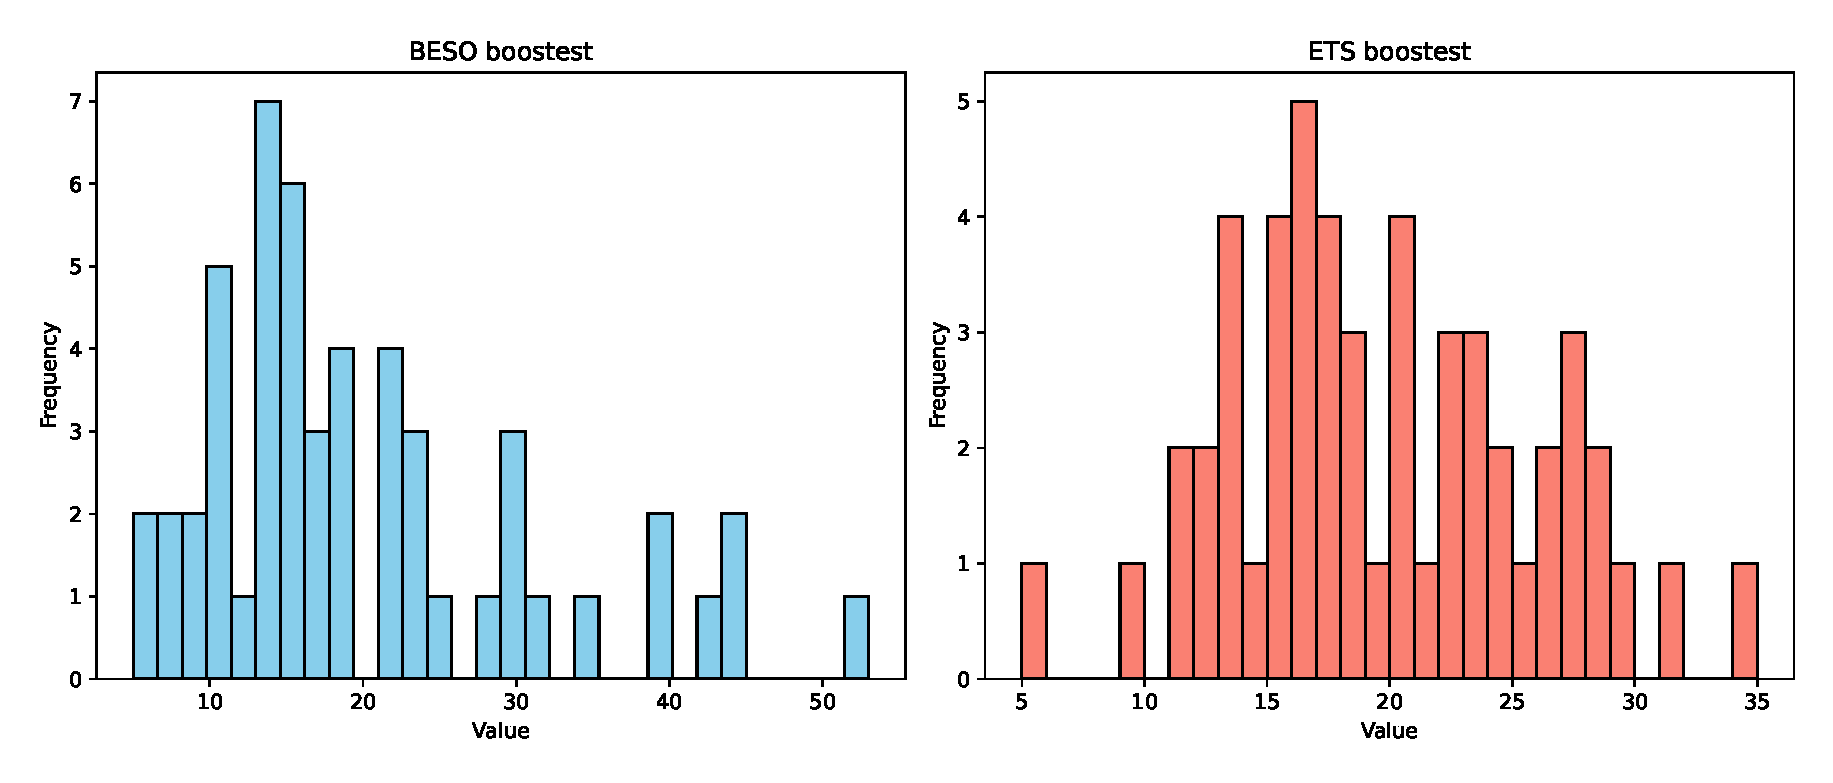
\includegraphics[width=0.75\linewidth]{compDistr.eps}%
    \caption{Comparison of distributions on 75 bootstrapped series}
    \label{fig:compDistr75}
\end{figure*}

The wider distribution has an impact on the proposed allocation. We had empirical proof of this when we tested the BESO and ETS solutions on the validation data obtained by the end of the year — i.e. when we finally received the data on which we were asked to provide a forecast.

Table ref{table:compETS} presents a comparison of solutions in the first two columns when no rental cost was added for the use of leased floor space and in the last two columns when the rental cost was included in the objective function. As expected, given that the constraints were less restrictive, the ETS solution is less expensive in both cases. However, in both cases, the solution was infeasible as it did not provide all the goods requested by one of the retailers. This result was obtained in a single instance; therefore, it may not have happened. However, it is significant that, even in the first instance in which we tested our model, its robustness proved important in dealing with a limit case.

\begin{table}
\centering
\begin{tabular}{l|cc|cc|}
& \multicolumn{2}{|c|}{No rental cost} & \multicolumn{2}{|c|}{With rental cost} \\
                 & BESO  & ETS   & BESO    & ETS     \\
\hline
Assign. Cost     & 17781 & 15423 & 5446720 & 4378380 \\
Optimality gap\% & 0     & 0     & 16.07   & 0.69    \\
Infeasibilities  & 0     & 1     & 0       & 1       \\
t.Cpu            & 33    & 29    & 3600    & 3600    \\
\hline
\end{tabular}
\caption{pitopiro}
\label{table:compETS}
\end{table}

Table \ref{table:resETS} details the proposed usage of the  DCs inthe different cases. It appears that DC 2, the biggest owned one, is the overloaded one in both cases, even though by small amounts. 

\begin{table}
\centering
\begin{tabular}{l|cc|cc|}
& \multicolumn{2}{|c|}{No rental cost} & \multicolumn{2}{|c|}{With rental cost} \\
                 & BESO  & ETS   & BESO    & ETS     \\
\hline
DC 0 & 67 / 120 & 119 / 120 & 82 / 120 & 116 / 120 \\
DC 1 & 571 / 1000 & 430 / 1000 & 532 / 1000 & 428 / 1000 \\
DC 2 & 257 / 300 & 301 / 300 & 257 / 300 & 303 / 300 \\
DC 3 & 128 / 180 & 173 / 180 & 152 / 180 & 176 / 180 \\
\hline
\end{tabular}
\caption{piropiro}
\label{table:resETS}
\end{table}

Finally, we note that Table \ref{table:compETS} shows that including the rental cost makes otherwise identical instances much harder to solve. In fact, the time limit of 3600 CPU seconds was too short to reach optimality, and a duality gap was left in the proposed solutions, a substantial one in the case of the BESO instance.

\subsection{Extended deterministic benchmark set} \label{Subsec:extend}

All analyses reported in sections \ref{Subsec:predictive} and \ref{Subsec:prescriptive} refer to the case study at the heart of this paper, but the interest of the method is not limited to this particular case study as it can be effective on any instance of this 2-echelon supply chain problem. To test the generality of the results, we generated a benchmark set with varying dimensions and coefficients. The study was conducted only with respect to the deterministic setting, and is therefore significant for assessing the computational complexity of the split-allocation problem as a deterministic combinatorial optimization problem.

We generated 5 instances for each configuration of number of clients ($n$), number of servers ($m$), and number of splittable clients. The travel costs were obtained by randomly selecting $m$ rows and $n$ columns from a large distance matrix, whose values were computed as the actual road distances between points located in the same area as the test case. Server inventory costs were inversely proportional to the average travel cost from the server to the clients and client requests were inversely proportional to the average travel cost from the client to the servers (note that the distance matrix is asymmetric being computed within a city area). The number $n_b$ of splittable clients was progressively increased as the number $n_q$ of servers with nonzero inventory costs. Specifically, the range of the defining parameters were:
\begin{itemize}
    \item $n$: \{50, 52, 100, 200, 300\};
    \item $m$: \{4, 5, 10, 25, 50\};
    \item $n_b$: \{0, 4, 5, 10, 25, 50\}
    \item $n_q$: \{0, 1, 2, 3, 4, 5\}
\end{itemize}

Not all combinations of values were generated, the larger values were used only for instances with higher number of clients. In particular, the values 4 and 52 were only used to generate instances with the same dimensionality as the case study, in order to check the generality of the results obtained. The first instance of this set was kept to be the case study one.

The computational results in the case of no costly server, reported as averages over the 5 generated instances, are summarized in table \ref{table:extset}, whose columns show:
\begin{itemize}
    \item $n$, $m$: number of clients and number of servers;
    \item $n_b$: maximum number of splittable clients;
    \item $ncols$, $nrows$: number of columns and number of rows in formulation FD;
    \item $gaplb$: average percentage gap between the linear relaxation lower bound and the cost of the best solution found;
    \item $gapfinal$: average percentage gap between the best lower bound at the end of the search (smallest cost of an unexpanded node) and the cost of the best solution found;
    \item $ninf$: number of instances for which no feasible solution was found;
    \item $nopt$: number of instances solved to proven optimality;
    \item $tcpu$: average CPU time for solving the instance, time to optimality or 3600 if optimality could not be proven;
\end{itemize}

\begin{table}
\centering
\renewcommand{\arraystretch}{0.75}
\begin{tabular}{cccccccccc}
$n$ & $m$ & $n_b$ & $ncols$ & $nrows$ & $gaplb$ & $gapfinal$ & $ninf$ & $nopt$ & $tcpu$\\
\hline
 52 &  4 &  0 &   416 &   316 & 0.21 & 0.01 & 0 & 5 &    0  \\
\hline
 50 &  5 &  0 &   500 &   355 & 0.39 & 0.00 & 0 & 5 &    3  \\
 50 &  5 &  5 &   500 &   355 & 0.40 & 0.00 & 0 & 5 &    4  \\
 50 & 10 &  0 &  1000 &   610 & 1.32 & 0.00 & 0 & 5 &  383  \\
 50 & 10 &  5 &  1000 &   610 & 1.34 & 0.00 & 0 & 5 &  378  \\
 50 & 10 & 10 &  1000 &   610 & 1.35 & 0.13 & 0 & 4 & 1150  \\
\hline
100 & 10 &  0 &  1000 &  1210 & 0.50 & 0.12 & 0 & 2 & 1920  \\
100 & 10 &  5 &  1000 &  1210 & 0.54 & 0.05 & 0 & 3 & 1514  \\
100 & 10 & 10 &  1000 &  1210 & 0.57 & 0.09 & 0 & 3 & 2063  \\
100 & 50 &  0 & 10000 &  5250 & 5.23 & 3.06 & 0 & 0 & 3600  \\
100 & 50 &  5 & 10000 &  5250 & 4.77 & 2.70 & 0 & 0 & 3600  \\
100 & 50 & 10 & 10000 &  5250 & 4.55 & 2.42 & 0 & 0 & 3600  \\
100 & 50 & 25 & 10000 &  5250 & 4.52 & 2.61 & 0 & 0 & 3600  \\
\hline
200 & 10 &  0 &  4000 &  2410 & 0.17 & 0.05 & 0 & 2 & 2369  \\
200 & 10 &  5 &  4000 &  2410 & 0.17 & 0.09 & 0 & 1 & 2893  \\
200 & 10 & 10 &  4000 &  2410 & 0.18 & 1.01 & 0 & 0 & 3600  \\
200 & 50 &  0 & 20000 & 10450 & 1.66 & 1.26 & 0 & 0 & 3600  \\
200 & 50 & 10 & 20000 & 10450 & 1.68 & 1.29 & 0 & 0 & 3600  \\
200 & 50 & 25 & 20000 & 10450 & 1.71 & 1.37 & 0 & 0 & 3600  \\
\hline
300 & 10 &  0 &  6000 &  3610 & 0.09 & 0.03 & 0 & 3 & 1798 \\
300 & 10 &  5 &  6000 &  3610 & 0.09 & 0.07 & 0 & 0 & 3600 \\
300 & 10 & 10 &  6000 &  3610 & 1.02 & 0.47 & 0 & 0 & 3600 \\
300 & 50 &  0 & 30000 & 15650 & 0.94 & 0.73 & 0 & 0 & 3600  \\
300 & 50 & 10 & 30000 & 15650 & 0.93 & 0.76 & 0 & 0 & 3600  \\
300 & 50 & 25 & 30000 & 15650 & 0.96 & 0.84 & 0 & 0 & 3600  \\
\hline
\end{tabular}
\caption{Extended benchmark set, deterministic case, no costly server}
\label{table:extset}
\end{table}

The table shows two trends. One, with respect to instance size, shows an expected increase in complexity. While instances the size of our test case are easily solved to optimality by modern solvers, increasing the size, as defined by the number of variables and the number of constraints, quickly leads to instances that could not be solved to optimality within the 3600-second time limit. 
The number of splittable clients has an important effect on the complexity of the instance. Instances of the same absolute size, but with more splittable clients, usually have a looser linear relaxation (LP) bound and have more difficulty reaching optimality, as can be seen by the decreasing number of instances out of the 5 from each group that could be solved to optimality.

Note that the optimality gap of the LP bound is usually small, except for the $n$=100 and $m$=50 instances, but the search still struggles to close this gap. Interestingly, the LP bound gets tighter as $n$ increases, but this does not make the search any easier.
The least-cost solution when optimality was not proven was usually found within the first 600 seconds of CPU time. However, we note that designing efficient heuristics for this problem is beyond the scope of this research. We could have tweaked the solver configuration to favor heuristic search at the expense of efficiency in proving optimality, or designed custom heuristics, but the focus here is on assessing the fitness landscape when road network costs are involved.

Table \ref{table:extsetq} reports results about tests varying the number of costly servers, the columns show:
\begin{itemize}
    \item $n$, $m$: number of clients and number of servers;
    \item $ncols$, $nrows$: number of columns and number of rows in formulation FD;
    \item lb0, t0: linear relaxation bound and CPU time in the case of no costly servers;
    \item lb1, t1: linear relaxation bound and CPU time in the case of 1 costly server;
    \item lb2, t2: linear relaxation bound and CPU time in the case of 2 costly servers;
    \item lb3, t3: linear relaxation bound and CPU time in the case of 3 costly servers;
    \item lb4, t4: linear relaxation bound and CPU time in the case of 4 costly servers;
    \item lb5, t5: linear relaxation bound and CPU time in the case of 5 costly servers;
\end{itemize}

The table reports results on two sets of instances. The top 4 rows contain aggregate results on a set of instances, 5 for each configuration, where inventory costs are directly proportional to average travel distances, while the bottom 4 rows have inventory costs inversely proportional to average travel distances.

\begin{table}
\addtolength{\tabcolsep}{-3pt}
\footnotesize 
\centering
\renewcommand{\arraystretch}{1.2}
\begin{tabular}{cccc|cc|cc|cc|cc|cc|cc}
n & m & ncols & nrows & lb0 & t0 & lb1 & t1 & lb2 & t2 & lb3 & t3 & lb4 & t4 & lb5 & t5 \\
\hline
52 & 4  & 416 & 316 & 0.86 & 0.2 & 0.17 & 0.81 & 0.08 & 0.22 & 0.01 & 0.02 & 0.00 & 0.02 & - & - \\
50 & 5  & 500 & 355 & 1.33 & 0.06 & 2.77 & 0.06 & 1.46 & 0.13 & 0.11 & 14.31 & 0.06 & 7 & 0.05 & 0.93 \\
100 & 5 & 1000 & 705 & 0.41 & 0.24 & 0.09 & 6.39 & 0.06 & 3.2 & 0.01 & 0.06 & 0.02 & 4.8 & 0.02 & 2.71 \\
200 & 5 & 2000 & 1405 & 0.14 & 1.43 & 0.01 & 1.79 & 0.01 & 0.25 & 0.01 & 0.17 & 0.01 & 0.11 & 0.01 & 7.84 \\
\hline
52 & 4  & 416 & 316 & 0.86 & 0.36 & 0.24 & 0.22 & 0.22 & 0.14 & 0.26 & 0.09 & 0.05 & 1.9 & - & - \\
50 & 5  & 500 & 355 & 1.33 & 0.16 & 0.52 & 0.07 & 0.50 & 5.8 & 0.13 & 10.11 & 0.05 & 1.37 & 0.02 & 0.22 \\
100 & 5 & 1000 & 705 & 0.41 & 0.33 & 0.19 & 8.58 & 0.04 & 6.14 & 0.02 & 0.41 & 0.02 & 0.58 & 0.02 & 3.78 \\
200 & 5 & 2000 & 1405 & 0.14 & 1.55 & 0.07 & 39.07 & 0.04 & 9.44 & 0.01 & 0.12 & 0.02 & 4.48 & 0.01 & 6.66 \\
\hline
\end{tabular}
\caption{Extended benchmark set, deterministic case, increasing number of costly servers}
\label{table:extsetq}
\end{table}

For both increasing and decreasing inventory costs, the complexity of solving instances increases nonmonotonically with the number of costly servers. In fact, while the 0 costly instances are comparatively easy to solve, the CPU time to prove optimality increases with the first costly servers, and then decreases as more servers are paid to store inventory. Interestingly, this is not true for the gap between the linear relaxation bound and the optimal solution cost, where the 0 costly instances always have the largest gap.
It is also not surprising that the CPU time required for proving optimality in all cases increases with the dimension of the case, and that the case with an inverse correlation between storage cost and travel cost is more difficult to solve than the case with a positive correlation.

% \section{Conclusions and future directions} \label{Sec:conclusions}

%The paper describes a case study in distribution logistics where retail stores need to be allocated to DCs in order to minimize allocation costs and to estimate inventory requests at the DCs. The retailer requests have to be forecast based on historical data series.

%The study calls for an approach that integrates forecasting and optimization. We proposed to ground the forecasting phase on bootstrapped autoregressive models, which, in addition to possessing properties particularly suited for integration with the subsequent optimization phase, also showed an effectiveness that was confirmed by computational comparisons with alternative forecasting methods.

%Bootstrapped forecasting allows the identification of a probability distribution of future retailer requests, which can be used to support stochastic optimization of allocations, taking into account both allocation costs and uncertainty in the forecasts.

%The combinatorial optimization problem at the core of the stochastic optimization module is a split allocation problem, which has been studied in the literature mainly in the design of survivable networks, in its deterministic version. On the contrary, we conducted a study on the fitness landscape of the problem when defined on transportation logistics data and in a stochastic context, obtaining results on the increase of complexity deriving from the variation of different parameters defining the problem instances.

%We believe that this study is of wide interest, both because it is an innovative case of predictive analytics and because the forecasting methodology presented, Maximum Entropy Bootstrap (MEB), offers justified insights that are of particular interest from a managerial perspective.

%This case study also provides the backbone for more detailed analysis. In fact, there are several directions in which the study can be extended. For example, we were interested in the optimal solution of the deterministic problems encountered, but an analysis of the effectiveness of heuristics may be of interest to managers. We solved the stochastic problem via its deterministic equivalent, but other stochastic optimization techniques may provide results that offer different perspectives on the case.

%Future research could also explore the integration of MEB methods within the preprocessing procedures usually needed in real life scenarios, e.g., of the type Box-Cox, to enhance predictive accuracy of the  algorithms considered. Additionally, examining various ensemble methods, including forecast combination techniques such as weighted averaging or regression-based methods, could yield valuable insights into achieving more robust predictions in highly variable environments. The interplay between predictive analytics and real-time decision-making processes warrants investigation, particularly how dynamic reallocation strategies informed by bootstrapped predictions impact overall logistics efficiency. Furthermore, extending the analysis to incorporate newly proposed machine learning algorithms could provide fresh perspectives on improving forecasting accuracy and operational flexibility, thereby fostering innovative solutions in logistics management.
%Finally, the closure properties of the MEB framework present opportunities for further enhancements, such as the integration of Bayesian prior information, which could refine estimations by incorporating external knowledge into the constraint mechanism. The exploration of hybrid models that merge Bayesian updating with maximum entropy principles may lead to richer representations of uncertainty and enhanced predictive accuracy. 

% the whole section starting from line 643 (Conclusions and future directions) is replaced as below reported


\section{Conclusions and future directions} \label{Sec:conclusions}

This paper builds on a case study in distribution logistics to propose a more general framework for prescriptive analytics called Bootstrap Enhanced Scenario Optimization (BESO). The case study is based on a 2-echelon supply chain where retail stores are allocated to distribution centers (DCs). The problem we analyzed was to minimize the allocation cost and the corresponding aggregated demand to each DC when the retailer requests are forecast based on historical data. This process allows us to ultimately determine the inventory required to be stocked in each DCs, and consequently the size needed to accommodate it. 

The study advocates integrating forecasting and optimization. We propose grounding the forecasting phase on bootstrapped autoregressive models, which demonstrated effectiveness compared to alternative methods. Bootstrapped forecasting identifies a probability distribution of future retailer requests, supporting stochastic optimization of allocations while considering both costs and forecast uncertainty. 

We considered both the cases where clients had to be fully allocated to a server and a split allocation version, and we  validated our framework using the transportation logistics data provided with the real-world use case and using artificial data for a better analysis of the fitness landscape revealing which defining parameters have the most impact on the instance complexity, obtaining results on the increase of complexity deriving from the variation of different parameters defining the problem instances.

We believe that this study is of wide interest, both because it is an innovative case of predictive analytics and because the framework composed by the forecasting methodology presented, Maximum Entropy Bootstrap (MEB), and deterministic equivalent based on the bootstrapped series, can be of particular interest from a managerial perspective because of the justified insights offered.

Future research could explore integrating MEB methods into preprocessing procedures, such as Box-Cox transformations, to enhance predictive accuracy. Additionally, investigating ensemble methods, including weighted averaging, may yield robust predictions in variable environments. The interplay between predictive analytics and real-time decision-making deserves attention, particularly regarding how strategies informed by bootstrapped predictions influence logistics efficiency. Lastly, the closure properties of the MEB framework allow for enhancements, such as incorporating Bayesian prior information, refining estimates by integrating external knowledge. Exploring hybrid models that merge Bayesian updating with maximum entropy may yield richer representations of uncertainty and enhanced predictive accuracy.

%\THEEndNotes
%\begingroup \parindent 0pt \parskip 0.0ex \def\enotesize{\normalsize} \theendnotes \endgroup

% Appendix here
% Options are (1) APPENDIX (with or without general title) or
%             (2) APPENDICES (if it has more than one unrelated sections)
% Outcomment the appropriate case if necessary
%
\begin{APPENDIX}{Bootstrap sets error costs} \label{app:errcost}
\clearpage % Ensures all pending floats are placed before this point

This section reports the absolute values of the different cost functions calculated on the forecast error obtained as an average of the corresponding errors on each of the 52 series of the test case described in the paper.

The functions reported in the columns are: bias, Means Absolute Percentage Error (MAPE), Mean Error (ME), Mean Absolute Error (MAE), Mean Percentage Error (MPE) and Root Mean Square Error (RMSE). Table \ref{table:app75} gives the cost values for the case of a boost set composed of 75 series, table \ref{table:app125} for the 125 series and table \ref{table:app175} for the 175 series sets.

All tables show significantly consistent results across all boost set sizes.

\begin{table}
\centering
\renewcommand{\arraystretch}{0.75}
\begin{tabular}{ccccccc}
model & bias & MAPE & ME & MAE & MPE & RMSE \\
\hline
fcast\_50   &-0.27 & 0.09 &-1.02 & 1.63 &-0.05 &  2.12 \\
fcast\_avg  & 0.02 & 0.07 & 0.07 & 1.25 & 0.01 &  1.68 \\
yar         & 0.36 & 0.34 & 1.36 & 5.86 & 0.07 &  9.75 \\
yhw         & 0.63 & 0.34 & 2.41 & 5.99 & 0.13 & 10.59 \\
ysvm        & 0.69 & 0.36 & 2.66 & 6.20 & 0.14 & 10.99 \\
ylstm       & 0.56 & 0.35 & 2.13 & 6.01 & 0.11 & 10.41 \\
ymlp        & 0.47 & 0.36 & 1.79 & 6.26 & 0.09 & 10.60 \\
yrf         & 1.50 & 0.44 & 5.73 & 7.79 & 0.31 & 13.54 \\
yxgb        & 2.28 & 0.58 & 8.74 &10.12 & 0.49 & 17.05 \\
yarima      & 0.44 & 0.34 & 1.67 & 5.80 & 0.09 &  9.77 \\
\hline
\end{tabular}
\caption{Error costs for the 75 series boostset.}
\label{table:app75}
\end{table}

\begin{table}
\centering
\renewcommand{\arraystretch}{0.75}
\begin{tabular}{ccccccc}
model & bias & MAPE & ME & MAE & MPE & RMSE \\
\hline
fcast\_50   & -0.56 & 0.09 & -1.08 & 1.59 & -0.06 & 2.25  \\
fcast\_avg  &  0.02 & 0.07 &  0.05 & 1.18 &  0.01 & 1.65  \\
yar         & -0.59 & 0.25 & -1.13 & 4.36 & -0.07 & 6.31  \\
yhw         & -0.13 & 0.24 & -0.26 & 4.33 & -0.02 & 6.39  \\
ysvm        & -0.06 & 0.24 & -0.11 & 4.18 & -0.01 & 6.39  \\
ylstm       & -0.30 & 0.24 & -0.58 & 4.15 & -0.04 & 6.34  \\
ymlp        & -0.47 & 0.24 & -0.90 & 4.22 & -0.05 & 5.99  \\
yrf         &  1.27 & 0.28 &  2.44 & 5.01 &  0.14 & 7.48  \\
yxgb        &  2.52 & 0.38 &  4.85 & 6.52 &  0.28 & 9.46  \\
yarima      & -0.40 & 0.25 & -0.76 & 4.44 & -0.05 & 6.83  \\
\hline
\end{tabular}
\caption{Error costs for the 125 series boostset.}
\label{table:app125}
\end{table}

\begin{table}
\centering
\renewcommand{\arraystretch}{0.75}
\begin{tabular}{ccccccc}
model & bias & MAPE & ME & MAE & MPE & RMSE \\
\hline
fcast\_50  & -0.04 & 0.07 & -0.07 & 1.22 & 0     & 1.51 \\
fcast\_avg & 0.99  & 0.12 & 1.90  & 2.04 & 0.12  & 2.76 \\
yar        & -0.22 & 0.35 & -0.42 & 5.84 & -0.03 & 7.64 \\
yhw        & 0.25  & 0.34 & 0.48  & 5.75 & 0.02  & 7.90 \\
ysvm       & 0.30  & 0.33 & 0.58  & 5.66 & 0.03  & 7.76 \\
ylstm      & 0.10  & 0.34 & 0.20  & 5.76 & 0     & 7.74 \\
ymlp       & -0.19 & 0.34 & -0.36 & 5.69 & -0.02 & 7.57 \\
yrf        & 1.72  & 0.37 & 3.31  & 6.39 & 0.18  & 9.66 \\
yxgb       & 3.01  & 0.46 & 5.78  & 7.96 & 0.33  & 11.83\\
yarima     & -0.04 & 0.34 & -0.08 & 5.69 & -0.01 & 7.63 \\
\hline
\end{tabular}
\caption{Error costs for the 175 series boostset.}
\label{table:app175}
\end{table}
\end{APPENDIX}
%
%   or
%
% \begin{APPENDICES}
% \section{<Title of Section A>}
% \section{<Title of Section B>}
% etc
% \end{APPENDICES}

% Acknowledgments here
%\ACKNOWLEDGMENT{We would like to express our sincere gratitude to [acknowledge individuals, organizations, or institutions] for their invaluable contributions to this research. We are also grateful to [mention any additional acknowledgements, such as technical assistance, data providers, or colleagues] for their support and assistance throughout the course of this work.}


% References here (outcomment the appropriate case)
% CASE 1: BiBTeX used to constantly update the references
%   (while the paper is being written).
%\bibliographystyle{informs2014} % outcomment this and next line in Case 1
%\bibliography{<your bib file(s)>} % if more than one, comma separated
\bibliographystyle{informs2014} 
\bibliography{GDObiblio}

%%%%%%%%%%%%%%%%%
\end{document}
%%%%%%%%%%%%%%%%%
